\documentclass[a4paper,twoside=false]{scrbook} 
\usepackage{etex}					% Avoid errors caused by too many packages
\usepackage[british]{babel}		% Correct Norwegian and English hyphenation
\selectlanguage{british}
\usepackage[utf8]{inputenc}			% Allow for non-ASCII input
\usepackage[T1]{fontenc}				% Use rich fonts
\usepackage{amsmath}
\usepackage{amssymb}
\usepackage[style=english]{csquotes}		% Context sensitive quotes
\usepackage{lmodern}				% Exploit the above

% Use classic (Computer Modern) fonts for headers
\setkomafont{disposition}{\normalfont\bfseries}
\addtokomafont{chapterprefix}{\huge}
\addtokomafont{chapter}{\Huge}

\usepackage{geometry}				% Better geometry

\sloppy							% better line breaks
\usepackage{microtype}

\setcounter{tocdepth}{3}

%%%%%%%%%%%%%%%%%%%%%%%%%%%%%%%%%%%%%%%%%%%%%%%%%%%%%
% Graphics, tables and figures
\usepackage{graphicx}                           
\usepackage[table]{xcolor}
\usepackage{colortbl}
\usepackage{tcolorbox}
\usepackage{framed}
\usepackage{tabularx}
\usepackage{multicol}
\usepackage{multirow} 
\usepackage{rotating}
\usepackage{array} 
\usepackage{supertabular}
\usepackage{hhline} 
\usepackage{subcaption}
\usepackage[shortlabels]{enumitem}
\usepackage{datatool}
\usepackage{amsmath}
\DeclareMathOperator*{\argmax}{argmax} % thin space, limits underneath in displays


\DTLloaddb{literature_study}{../documents/literature_study.csv}


% pdf stuff
\usepackage{pdfpages} 
% \usepackage{fancyhdr}
\usepackage{afterpage}

% nicer table dividers á la MIT Press; the package booktabs provides a similar option
\usepackage{booktabs}
% \newcommand\tabletop{\hline\noalign{\smallskip}}
% \newcommand\tablemid{\noalign{\smallskip}\hline\noalign{\smallskip}}
% \newcommand\tablebot{\noalign{\smallskip}\hline}

% only needed if you want to pgfplots to draw figures
\usepackage{tikzsymbols}
\usepackage{pgfplots}
\pgfplotsset{compat=1.16}

%%%%%%%%%%%%%%%%%%%%%%%%%%%%%%%%%%%%%%%%%%%%%%%%%%%%%
% URLs and hyperlinks
\usepackage[hyphens]{url}
\usepackage{doi}
\usepackage{hyperref}
\definecolor{darkblue}{rgb}{0, 0, 0.5}
\hypersetup{colorlinks=true,citecolor=black, linkcolor=black, urlcolor=darkblue}
\usepackage[nameinlink]{cleveref}

\let\oldFootnote\footnote
\newcommand\nextToken\relax

\renewcommand\footnote[1]{%
    \oldFootnote{#1}\futurelet\nextToken\isFootnote}

\newcommand\isFootnote{%
    \ifx\footnote\nextToken\textsuperscript{,}\fi}

% Code stuff
\usepackage{listings}

\definecolor{dkgreen}{rgb}{0,0.6,0}
\definecolor{gray}{rgb}{0.5,0.5,0.5}
\definecolor{mauve}{rgb}{0.58,0,0.82}

\lstdefinestyle{yaml}{
    frame=tb,
    basicstyle=\color{darkblue}\footnotesize,
    rulecolor=\color{black},
    string=[s]{'}{'},
    stringstyle=\color{darkblue},
    comment=[l]{:},
    commentstyle=\color{black},
    morecomment=[l]{-},
    columns=flexible
}

\lstdefinestyle{python}{
    language=Python, breaklines=True, 
}

%%%%%%%%%%%%%%%%%%%%%%%%%%%%%%%%%%%%%%%%%%%%%%%%%%%%%
% comments and notes, useful while working on a draft - change the option 'draft' to 'disable' in the final version
\setlength{\marginparwidth}{2cm}
\usepackage[draft,textsize=footnotesize,textwidth=15mm]{todonotes}
%\usepackage[disable]{todonotes}

\usepackage{verbatim}				% allow for longer comments
%TC:group comment 0 0'

%%%%%%%%%%%%%%%%%%%%%%%%%%%%%%%%%%%%%%%%%%%%%%%%%%%%%
% BIBLIOGRAPHY STUFF

% \usepackage[round]{natbib}

\def\BibTeX{\textrm{B\kern-.05em\textsc{i\kern-.025em b}\kern-.08em T\kern-.1667em\lower.7ex\hbox{E}\kern-.125emX}}

% uncomment if instead using biber as backend
% \begin{comment}
\usepackage[backend=biber,
            bibstyle=apa,
            citestyle=authoryear,
            natbib=true,
            url=true,
            doi=true,
            hyperref=true,
            apamaxprtauth=99,
            maxcitenames=2,
            language=british,
            uniquelist=false,
            ]{biblatex}         				% Correct citations 

% Bibliography (+ hacks)
% \addbibresource{bib/references.bib}
\addbibresource{bib/bibliography.bib}  
\DeclareLanguageMapping{british}{british-apa}
\setlength\bibitemsep{2\itemsep}
\patchcmd{\bibsetup}{\interlinepenalty=5000}{\interlinepenalty=10000}{}{}
\let\citep\parencite
\let\cite\textcite
% Make the whole cite a hyperref
\DeclareCiteCommand{\textcite}
{\boolfalse{cbx:parens}}
{\usebibmacro{citeindex}%
    \printtext[bibhyperref]{\usebibmacro{textcite}}}
{\ifbool{cbx:parens}
    {\bibcloseparen\global\boolfalse{cbx:parens}}
    {}%
    \multicitedelim}
{\usebibmacro{textcite:postnote}}
\DeclareCiteCommand{\parencite}[\mkbibparens]
{\usebibmacro{prenote}}
{\usebibmacro{citeindex}%
    \printtext[bibhyperref]{\usebibmacro{cite}}}
{\multicitedelim}
{\usebibmacro{postnote}}
% \end{comment}

%%%%%%%%%%%%%%%%%%%%%%%%%%%%%%%%%%%%%%%%%%%%%%%%%%%%%
% HYPHENATION DEFINITIONS

\usepackage{hyphenat}
 
% add correct hyphenations as needed
\hyphenation{hash-tag Sem-Eval}
\hyphenation{cyber-bully cyber-bullying}

% Utility commands
\newcommand{\Autochapterref}[1]{\hyperref[#1]{Chapter~\ref*{#1}}}
\newcommand{\Autosectionref}[1]{\hyperref[#1]{Section~\ref*{#1}}}
\newcommand{\Autosubsectionref}[1]{\hyperref[#1]{Subsection~\ref*{#1}}}
\newcommand{\Autosubsubsectionref}[1]{\hyperref[#1]{Subsubsection~\ref*{#1}}}
\newcommand{\rqref}[1]{\hyperref[#1]{RQ\ref*{#1}}}

% \newcommand{\includeappendixpdf[2]{
%     \includepdf[pages=#1, scale=.7, pagecommand={\chapter{#1}\label{pdf:myfile}}, linktodoc=true]{#2}  
% }

\newcommand{\includeappendixpdfwithtitle}[3]{
    \newgeometry{top=.5in}
    \includepdf[pages=1, scale=.7, pagecommand={\chapter{#1}\label{#3}}, linktodoc=true]{#2}
    \restoregeometry
    \includepdf[pages=2-, scale=.7, pagecommand={}, linktodoc=true]{#2}
  }

% Styling 
\usepackage{setspace}
\usepackage{etoolbox}
\AtBeginEnvironment{quote}{\par\singlespacing\small}

\newcolumntype{B}{>{\bfseries}c}

%%%%%%%%%%%%%%%%%%%%%%%%%%%%%%%%%%%%%%%%%%%%%%%%%%%%%
% Acronym stuff
\usepackage[
nonumberlist, 			% if you don't want to show pagenumbers 
toc, 					% entry in the table of contents; can be left out
acronym] 				% create a list of abbreviations
{glossaries}
\usepackage[acronym]{glossaries}
\makeglossaries
\loadglsentries[main]{frontmatter/glossary.tex}

%%%%%%%%%%%%%%%%%%%%%%%%%%%%%%%%%%%%%%%%%%%%%%%%%%%%%
% Author
% Fill in here, and use these commands in the text.
\newcommand{\thesisAuthor}{Karl Oskar Magnus Holm} 
\newcommand{\thesisTitle}{LLMs - The Death of GIS Analysis?}
\newcommand{\thesisSubtitle}{An Investigation into Using Large Language Models for GIS Data Analysis}
\newcommand{\thesisType}{Specialization Project in Computer Science and Geomatics}
\newcommand{\supervisor}{Supervisor at NTNU: Hongchao Fan}
\newcommand{\externalSupervisors}{External supervisors from Norkart: Alexander Salveson Nossum, Arild Nomeland, and Rune Aasgaard}
\newcommand{\thesisDate}{December 2023}

\graphicspath{ {./figs/} }

%%%%%%%%%%%%%%%%%%%%%%%%%%%%%%%%%%%%%%%%%%%%%%%%%%%%%
% In case you don't want to compile all the LaTeX files every time, 
% you can list the ones you're currently working on here and compile those only.

% \includeonly{chapters/architecture} 

%%%%%%%%%%%%%%%%%%%%%%%%%%%%%%%%%%%%%%%%%%%%%%%%%%%%%
\begin{document}

%Title page (generated automatically from the commands above)
%This title page isn't strictly necessary and can be commented out if you don't want it
%\begin{comment}
\pagenumbering{alph}
\begin{titlepage}
    \noindent {\large \textbf{\thesisAuthor}}
    \vspace{2cm}

    \noindent {\Huge \thesisTitle}
    \vspace{5mm}

    \noindent {\huge \thesisSubtitle}
    \vspace{2cm}

    \noindent \thesisType, \thesisDate \newline
    \noindent \supervisor \newline
    \noindent \externalSupervisors
    \vspace{2cm}

    % \noindent Data and Artificial Intelligence Group\\
    \noindent Department of Geomatics\\
    Faculty of Engineering\\
    Norwegian University of Science and Technology\\

    \vfill
    \begin{center}
        
\includegraphics[width=3cm]{NTNUlogo.pdf}
    \end{center}
    \thispagestyle{empty}
\end{titlepage}

\clearpage
%\end{comment}   %Needed if commenting out the titlepage

%%%%%%%%%%%%%%%%%%%%%%%%%%%%%%%%%%%%%%%%%%%%%%%%%%%%%
\frontmatter

\addcontentsline{toc}{chapter}{Abstract}    % can be left out
\section*{Abstract}
This paper provides a template for writing a Master's Thesis 
(parts of it can also be used when writing a Specialisation Project Report). 
The template does not form a compulsory style that you are obliged to use, but rather provides a common starting point for all students. For a given thesis, tuning of the template may still be required, depending on the nature of the thesis and the author's writing style. 
Such tuning might involve moving a chapter to a section or vice versa, or removing or adding sections and chapters.

[If you write a Specialisation Project Report, it should normally focus on the background, related work (i.e., your literature study), and future work sections --- 
with the ``future work'' section containing the plan for the Master's Thesis work to be carried out in the second semester. 
Architectural and experimental sections can also be included, but in preliminary versions. 
All those sections should of course be updated in the Master's Thesis and adapted to the actual work carried out.]

Note that the template contains a lot of examples of how to write different parts of the thesis 
as well as how to cite authors and how to use LaTeX and BibTeX. 
Some of those examples might only be clear if you actually look at the LaTeX source itself.

The abstract is your sales pitch which encourages people to read your work, 
but unlike sales it should be realistic with respect to the contributions of the work. 
It should include:
\begin{itemize}
\item the field of research,
\item a brief motivation for the work,
\item what the research topic is, 
\item the research approach(es) applied, and 
\item contributions.
\end{itemize}

The abstract length should be roughly half a page of text (and not more than one page). 
It will normally be longer than the abstracts you see in research papers, since some more background / motivation is included.
Do not include lists, tables or figures.
Avoid abbreviations and references. 

When writing the abstract, keep in mind that most people might only read this text (and many only the title), so be sure to make it sound good.
What you really want to accomplish is that people who read the abstract will get drawn into your project and read the rest of the text too.
However, the old saying most definitely applies here: You never get a second chance to make a first impression. 

% \addcontentsline{toc}{chapter}{Sammendrag}  % can be left out
% \begin{otherlanguage}{norsk}

    \section*{Sammendrag}

\end{otherlanguage}

\begin{comment}
Husk at hvis du er en norsk student og skriver masteren din på engelsk, så \textit{må\/} du lage et sammendrag på norsk.
Bruk ikke Google Translate eller lignende, uten skriv teksten direkte på norsk.
Sammendraget trenger absolutt ikke å være identisk ord-for-ord med abstract, men skal selvsagt ha i prinsipp samme innehold, på semantisk nivå.

(If you are a non-Norwegian student, it is not obligatory to include an abstract in Norwegian.)

For those who write a Norwegian summary, whatever you do, do \textit{not\/} just directly translate the English abstract.
It might be tempting to think that the Norwegian summary is something you can do on the fly --- maybe assuming that nobody will read it.
However, in fact the opposite might be true: it is very likely that it will be read by the people you most want to make a good impression on,
such as your friends, family, and future employers.
\end{comment}

% \addcontentsline{toc}{chapter}{Preface}     % can be left out
% \section*{Preface}

\begin{comment}
The Preface includes the facts: what type of project, where it is conducted,
who supervised, and any acknowledgements you wish to give.

This Master's Thesis template was created by Bj\"orn Gamb\"ack and is based on a template that he created for the 2016 ``Experts in Team'' course on
Computational Creativity (TDT4853) at the Norwegian University of Science and Technology (NTNU),
which in turn was heavily based on the 2014 AI Master's Thesis template created by Anders Kofod-Petersen ---
with some of the explaining text stemming from Anders' original template.

You may basically thank anybody you like (and avoid thanking anybody you do not like) and in any form you like.
However, it is a good idea to always thank people who made direct contributions, e.g., those whose data you have been given access to or those whose images you have been given permission to reproduce.

Some students choose to include the text of the original project description in the Preface. This is possible but not necessary,
in particular not if you have changed the theme somewhat over time.
The Preface of the Master's Thesis might also be a good place to introduce your Specialisation Project, in case you plan
on reusing some texts from it (since the Specialisation Project is not a published and easily accessible work, and might
not be known to your audience, neither your text in itself nor even the general concept as such).
\end{comment}

\vfill

\hfill \thesisAuthor

\hfill Trondheim, \today


\clearpage

\tableofcontents

\listoffigures
\addcontentsline{toc}{chapter}{List of Figures} % can be left out

\listoftables
\addcontentsline{toc}{chapter}{List of Tables} % can be left out

\glsaddall              % to include all glossary entries

%%%%%%%%%%%%%%%%%%%%%%%%%%%%%%%%%%%%%%%%%%%%%%%%%%%%%
\mainmatter

\chapter{Introduction}
\label{cha:introduction}

\begin{comment}
All chapters should begin with an introduction before any sections, giving an overview of the chapter content.
Each section should in addition start with an introduction before its subsections begin.
Chapters with just one section --- or sections with just one sub-section --- should be avoided.
Think carefully about chapter and section titles as each title stands alone in the table of contents (without associated text)
and should convey the meaning of the contents of the chapter or section.

In all chapters and sections it is important to write clearly and concisely. Avoid repetitions and if needed refer back to the original discussion or presentation.
Each new section, subsection or paragraph should provide the reader with new information and be written in your own words. Avoid direct quotes.
If you use direct quotes, unless the quote itself is very significant, you are conveying to the reader that you are unable to express this discussion or fact yourself.
Such direct quotes also break the flow of the language (yours to someone else's).
\end{comment}

\section{Background and Motivation}
\label{sec:BackgroundAndMotivation}

\begin{comment}
Having a template to work from provides a starting point.
However, for a given project, a slight variation in the template may be required due to the nature of the given project.
Furthermore, the order in which the various chapters and sections will be written will also vary from project to project,
but the writing will seldom start at the abstract and sequentially follow the chapters of the report.
One critical reason for this is that you need to start writing as early as possible and that you will begin to write up where you are currently focusing.
However, do not leave working on the abstract until the very last days. The abstract is the first thing anyone reads of an article or thesis --- after the title;
and thus it is important that it is very well written. Abstracts are hard to write, so create revisions throughout the course of your project.

The background and motivation here should state where your project is situated in the field and what the key driving forces motivating this research are.
However, keep this section brief, as it is still part of the introduction.
The motivation will be further elaborated on in Chapter~\ref{cha:related_work}, presenting your complete state-of-the-art.

Note that this template uses italics to highlight where Latin wording is inserted to represent text and the text of the template
that we wish to draw your attention to. The italics themselves are not an indication that such sections should use italics.
\end{comment}

% The field of \acfull{acr:llm}
The field of \glspl{acr:llm} is an emerging one. \cite[2]{fanLargeLanguageModels2023} found that the proportion of papers about \glspl{acr:llm}\footnote{Including articles whose title or abstract includes "LLM", "Large Language Model", or "GPT".} to arXiv has skyrocketed since 2020, with a six-times increase in percent points from 2022 to 2023. They write that prompt engineering has been extensively used as a way to improve code generation \citep[7]{fanLargeLanguageModels2023}

\section{Goals and Research Questions}
\label{sec:GoalsandResearchQuestions}

\begin{comment}
A research project needs to have one or several question(s) that should be answered.
It is desirable to formulate such questions as early as possible as they provide both an important driving force for the project and clarity as to the goals sought.
However, expect to refine the questions and thus the final path of the project as work progresses.
Any refinements should be conducted with care, so as to avoid that the original aims and previous work are lost.
It is always good to have one (or max two) research goals and perhaps some subgoals,
together with 2--3 explicit research questions (or max four).

\begin{description}
    \item[Goal] \textit{Lorem ipsum dolor sit amet, consectetur adipiscing elit.}
\end{description}

Your goal/objective should be described in a single sentence.
In the text underneath it you can expand on this sentence to clarify what is meant by the short goal description.
The goal of your work is what you are trying to achieve. This can either be the goal of your actual project or
can be a broader goal that you have taken steps towards achieving. Such steps should be expressed in the research questions.
Note that the goal is seldom to build a system. A system is built to enable experiments to be conducted.
The research goal stages the needs that the system is implemented to meet.

\begin{description}
    \item[Research question 1] \textit{Lorem ipsum dolor sit amet, consectetur adipiscing elit.}
\end{description}

Each research question provides a sub-goal and these should be precise and clearly stated enabling the reader to match your results to the original goals.
They will also form the driving force for the experimental plan.

\begin{description}
    \item[Research question 2] \textit{Lorem ipsum dolor sit amet, consectetur adipiscing elit.}
\end{description}

Potentially, how well the goals have been met (and how well the research questions have been answered)
is a theme that you should return to towards the end of the thesis (so in Chapter~\ref{cha:conclusion} and/or Chapter~\ref{cha:discussion}).

For a Specialisation Project, the goal would primarily be to get up to speed with the research field, so the research questions will rather be
limited to exploring what the state-of-the-art is, what methods and data have been used, etc.
A secondary goal of the specialisation is to frame the research questions and goals of the Master's Thesis.
Note that a major difference between the Specialisation Project and the Master's Thesis is that the Master's Thesis work \textit{has\/} to
introduce new research.
Of course the Specialisation Project can also introduce novel work, but there is no such requirement --- and most commonly it does not,
since the core of the project really is to figure out what is ``old'' before you can introduce something which is new.
\end{comment}

The overarching goal of this specialization project is to investigate how \acrfull{acr:llm} can be utilized to make \acrshort{acr:gis} analysis simpler, faster, and more accessible. As exemplified in the task description provided by Norkart (see \cref{app:task-description}), such a system should be able to create a meaningful response to a query such as:

\begin{quote}
    "Find all buildings within a 100-meter belt that are above 100 meters above sea level and have docks."
\end{quote}

The task then is to investigate how modern language models can be used to perform classical \acrshort{acr:gis} analyses using standard \acrshort{acr:gis} technologies like PostGIS and geospatial data catalogues adhering to \acrshort{acr:ogc} or \acrshort{acr:stac} standards. Based on the task description I have constructed three research questions that I will attempt to answer in this specialization project report:

\begin{enumerate}
    \item What is the potential of LLM-based GIS analysis? \label{rq:llm-potential}
    \item How can OGC API Features be used in an overlay analysis using ChatGPT-4? \label{rq:overlay-analysis}
    \item How can we give ChatGPT-4 access to external tools? \label{rq:external-tools}
\end{enumerate}

Researching the potential of using \glspl{acr:llm} in GIS could uncover new methodologies for spatial analysis, predictive modeling, and decision-making. The aim with \rqref{rq:llm-potential} would be to assess the capabilities and limitations of integrating machine learning algorithms with \glspl{acr:gis}, and also touch on how a mature \acrshort{acr:llm}-based \acrshort{acr:gis} could impact the daily work of (human) \acrshort{acr:gis} professionals.

\rqref{rq:overlay-analysis} focuses on the feasibility of using the \acrshort{acr:ogc} \acrshort{acr:api} - Features Standads in a typical overlay analysis within a conversational \acrshort{acr:ai} context like ChatGPT-4, having the users be able to express themselves using natural language queries. An answer to \rqref{rq:overlay-analysis} would describe how \acrshort{acr:ogc} \acrshortpl{acr:api} can be called and manipulated in a flexible manner during a conversation to perform spatial queries or analyses, like intersecting layers or filtering features based on certain criteria.

\rqref{rq:external-tools} delves into the technical and ethical considerations of expanding ChatGPT-4's capabilities through integration with external tools, such as \acrshort{acr:gis} software or data analytics platforms. It would explore options for secure and efficient data exchange, and assess the implications of such access in terms of data privacy and user consent.

\section{Research Method}
\label{sec:researchMethod}

\begin{comment}
What methodology will you apply to address the goals: theoretic/analytic, model/abstraction or design/experiment?
This section will describe the research methodology applied and the reason for this choice of research methodology.
You should return to the actual choices made in the work and the alternatives in the Discussion chapter.
\end{comment}

\subsection{Literature Study}\label{subsec:literature-study}

I set out by deciding on some search terms, and used a "snowball sampling" technique to find relevant articles. \autoref{tbl:literature-search-resutls} shows the number of search results on various sites.

\todo{Fix table data and styling}
\begin{table}
    \DTLdisplaydb{literature_study}
    \caption{Literature study search results.}
    \label{tbl:literature-search-resutls}
\end{table}

\section{Contributions}
\label{sec:introContributions}

\begin{comment}
This section just provides a brief summary of the main contributions of the work.
The main description of the contributions will come in Section~\ref{sec:contributions}, after the results are presented.
(Hence Section~\ref{sec:introContributions} can also be left out, leaving the discussion completely to Section~\ref{sec:contributions}.)

The format of this section will generally be as follows:

\begin{enumerate}
    \item \textit{Lorem ipsum dolor sit amet, consectetur adipiscing elit.}
    \item \textit{Lorem ipsum dolor sit amet, consectetur adipiscing elit.}
    \item \textit{Lorem ipsum dolor sit amet, consectetur adipiscing elit.}
\end{enumerate}

\noindent
where the items on the list briefly describe the key contributions.

The order of the contributions here is important. List your main contribution first!
Creating this list will help you not only with writing the Conclusion (where all items listed here definitely should be included, and in more detail),
but also with items that need to be mentioned in the Abstract, as well as with points that you will want to bring to attention in the Discussion.
Hence most of the content on this list will be addressed 4--5 times in your text: here, in the Abstract, Discussion, Conclusion, and (most likely)
in the Results chapter.
\end{comment}

\section{Thesis Structure}
\label{sec:thesisStructure}

\begin{comment}
This section provides the reader with an overview of what is coming in the next chapters.
You want to say more than what is explicit in the chapter name, if possible, but still keep the description short and to the point. So something along the lines of:

\begin{itemize}
    \item Chapter~\ref{cha:background_theory} introduces the theory, tools and methods necessary to understand the work.
    \item \textit{Lorem ipsum dolor sit amet, consectetur adipiscing elit.}
    \item Chapter~\ref{cha:conclusion} sums up the work and points to ways it can be improved or extended in the future.
\end{itemize}
\end{comment}

\glsresetall
\chapter{Theory}\label{cha:theory}

\begin{comment}
The background theory depth and breadth depend on the depth needed to understand your project
in the different disciplines that your project crosses.
It is not a place to just write about everything you know that is vaguely connected to your project.
The theory is here to help the readers that do not know the theoretical basis of your work so that they
can gain sufficient understanding to understand your contributions --- and also for yourself to show that
you have understood the underlying theory and are aware of the methods used in the field.
In particular, the theory section provides
an opportunity to introduce terminology that can later be used without disturbing the text with a definition.
In some cases it will be more appropriate to have a separate section for different theories (or even separate chapters).
However, be careful so that you do not end up with too short sections.
Subsections may also be used to separate different background theories.

Be aware that ``background'' is a general term that refers to everything done by somebody else,
in contrast to the ``foreground'', which is your own work.
Hence there can (and will) be several background chapters, with the background theory being one of them
--- or several of them, since it thus is quite possible to split the background theory over more than one chapter,
e.g., by having a chapter introducing the theory directly needed for the research field in question and another
chapter discussing the machine learning theory, algorithms, tools, and evaluation methods commonly used in the field.
The related work chapter is thus also part of the background, while a chapter about data might be background
(if you only use somebody else datasets), but can also be part of the foreground (if you collect and/or annotate data
yourself, or if you process or clean the data in ways that can make it part of your own contribution).

It is ok to reuse material from other texts that you have written (e.g., the specialisation project), but if you do so, that must be clearly stated in the text, together with a description of how much of the text is new, old or rewritten/edited.
Such a statement about recycling of material in the Background Theory chapter can thus come here in the chapter introduction.

\section{Writing References in the Text}
\label{sec:writing_references}

When introducing techniques or results, always reference the source.
Be careful to reference the original contributor of a technique and not just someone who happens to use the technique.%
\footnote{But always make sure that you have read the work you are citing --- if not, cite someone who has!}
For results relevant to your work,
you would want to look particularly at newer results so that you have referenced the most up-to-date work in your area.
A common rule of thumb is to at least reference the first paper introducing the issue and the paper containing the latest / state-of-the-art
results. Additional papers making substantial contributions should also be referenced, as well as of course the ones you find most interesting.
Remember to use the right verb form depending on the number of authors.

If you do not have the source handy when writing, mark in the text that a reference is needed and add it later. \todo{add reference}
Web pages are not reliable sources --- they might be there one day and removed the next; and thus should be avoided, if possible.
A verbal discussion is not a source and should normally not be referenced
(though you can reference ``personal communication'', if there are no other options).
The bulk of citations in the report will appear in Chapter~\ref{cha:related_work}.
However, you will often need to introduce some terminology and key citations already in this chapter.

You can cite a paper in the following manner (and several other versions,
see the \verb!natbib! package documentation):

\section{The Reference List}
\label{sec:reference_list}

In general, make sure that the references that appear in your reference list can be easily located and identified by the reader.
So include not only authors and title, but year and place of publication, the full names of conferences and workshops,
page numbers in proceedings and collections, etc.
Hyperlinks or \acrfull{acr:doi} numbers are also nice to include.
Just as in the text itself, it is important to be consistent in the reference list, so include the same type of information for all references and write it in the same way.

% Check out the reference list at the end of this document for examples of how to write references in \BibTeX.
% Note a particular quirk: Many \BibTeX\ styles convert uppercase letters to lowercase, unless specifically told not to.
% You might thus need to ``protect'' characters that should not be converted, e.g., by writing \texttt{\{T\}witter} as in the \citet{FountaEA:18} reference.

% Also, keep in mind that `et' is a word in its own right (`and'), so there is no period after it (even though there is a period after `al.', which is short for `alia', meaning `others').
% Of course, when including such a reference in the text, the authors should be referred to in plural form. 
% So \citet{BenyonEA:13} state that life is good (not ``states'').

% Many sites, such as journals and \url{dblp.org} provide the matching \BibTeX\ entry for a reference. 
% However, you might still need to edit the entry in order to be consistent with the rest of your references.
% If you find references from sites such as \url{scholar.google.com} or \url{arXiv.org}, keep in mind that they often not are complete,
% so that you might need to add information to the entry (and probably edit it as well).

Some other good sites to find state-of-the-art work:
\begin{itemize}
    \item \url{paperswithcode.com}
    \item \url{nlpprogress.com}

\end{itemize}

\textit{Lorem ipsum dolor sit amet, consectetur adipiscing elit, sed do eiusmod tempor incididunt ut labore et dolore magna aliqua. Ut enim ad minim veniam, quis nostrud exercitation ullamco laboris nisi ut aliquip ex ea commodo consequat. Duis aute irure dolor in reprehenderit in voluptate velit esse cillum dolore eu fugiat nulla pariatur. Excepteur sint occaecat cupidatat non proident, sunt in culpa qui officia deserunt mollit anim id est laborum.}


\section{Introducing Figures}

\LaTeX is a bit tricky when it comes to the placement of ``flooting bodies'' such as figures and tables. It is often a good idea to let their code appear right before the header of the (sub)section in which they appear.
Note that you should anyhow always use an option for the placement (e.g., \verb|[t!]| to place it at the top of a page).

Do not just put the figure in and leave it to the reader to try to understand what the figure is.
The figure should be included to convey a message and you need to help the reader to understand the message
intended by explaining the figure in the text.
Hence \textbf{all} figures and tables should always be referenced in the text, using the \verb!\ref! command.
It is good practice to always combine it with a non-breakable space (\verb!~!) so that there will be no newline between the term referring to it and the reference, that is, using \verb!Figure~\ref{fig:BoxesAndArrowsAreNice}!.

Also, note that you can have a longer version of the figure (and table) caption attached to the actual figure,
while using the optional first argument to \verb!\caption! to include a shorter version in the list of figures (lof) or list of tables:
\begin{quote}
    \begin{verbatim}
\caption[Shorter lof text]{Longer text appearing under the figure}
\end{verbatim}
\end{quote}

\begin{figure}[t!]
    \centering
    \missingfigure{Here we will add an amazing figure explaining it all}
    \caption{A missing figure}
    \label{fig:AmazingFigure}
\end{figure}

In general it is good to add notes about things that you plan on writing later.
The \verb!todonotes! package is great for that kind of book-keeping, letting you write both shorter comments in the margin\todo{l8r dude} and longer comments inside the text, using the option \verb![inline]!.
\todo[inline]{There are always some more stuff that you will need to add at some later point.
    Be sure to at least make a note about it somewhere.}

\textit{Sed ut perspiciatis unde omnis iste natus error sit voluptatem accusantium doloremque laudantium, totam rem aperiam, eaque ipsa quae ab illo inventore veritatis et quasi architecto beatae vitae dicta sunt explicabo. Nemo enim ipsam voluptatem quia voluptas sit aspernatur aut odit aut fugit, sed quia consequuntur magni dolores eos qui ratione voluptatem sequi nesciunt. Neque porro quisquam est, qui dolorem ipsum quia dolor sit amet, consectetur, adipisci velit, sed quia non numquam eius modi tempora incidunt ut.}

\section{Introducing Tables in the Report}

\newcommand\emc{-~~~~}
\begin{table}[t!]
    \centering
    \caption[Example table]{Example table (F$_1$-scores); this table uses the optional shorter caption that will appear in the list of tables, so this long explanatory text will not appear in the list of tables and is only here in order to explain that to the reader.}
    \begin{tabular}{c|c|rrrrrr}
        \tabletop
        Langs                  & Source                                           & \multicolumn{1}{c}{Lang1} & \multicolumn{1}{c}{Lang2} & \multicolumn{1}{c}{Univ} & \multicolumn{1}{c}{NE} & \multicolumn{1}{c}{Mixed} & \multicolumn{1}{c}{Undef}
        \\ \tablemid
        \multirow{5}{*}{EN-HI} & FB+TW                                            & 54.22                     & 22.00                     & 19.70                    & 4.00                   & 0.05                      & 0.03                      \\
                               & FB                                               & 75.61                     & 4.17                      & 18.00                    & 2.19                   & 0.02                      & 0.01                      \\
                               & TW                                               & 22.24                     & 48.48                     & 22.42                    & 6.71                   & 0.08                      & 0.07                      \\
                               & Vyas                                             & 54.67                     & 45.27                     & 0.06                     & \emc                   & \emc                      & \emc                      \\
                               & FIRE                                             & 45.57                     & 39.87                     & 14.52                    & \emc                   & 0.04                      & \emc                      \\ \tablemid
        \multirow{2}{*}{EN-BN} & TW                                               & 55.00                     & 23.60                     & 19.04                    & 2.36                   & \emc                      & \emc                      \\
                               & FIRE                                             & 32.47                     & 67.53                     & \emc                     & \emc                   & \emc                      & \emc                      \\ \tablemid
        EN-GU                  & FIRE                                             & 5.01                      & \textbf{94.99}            & \emc                     & \emc                   & \emc                      & \emc                      \\
        \tablemid
        DU-TR                  & Nguyen                                           & 41.50                     & 36.98                     & 21.52                    & \emc                   & \emc                      & \emc                      \\ \tablemid

        EN-ES                  & \multirow{4}{*}{\rotatebox[origin=c]{90}{EMNLP}}
                               & 54.79                                            & 23.50                     & 19.35                     & 2.08                     & 0.04                   & 0.24                                                  \\
        EN-ZH                  &                                                  & 69.50                     & 13.95                     & 5.88                     & 10.60                  & 0.07                      & \emc                      \\
        EN-NE                  &                                                  & 31.14                     & 41.56                     & 24.41                    & 2.73                   & 0.08                      & 0.08                      \\
        AR-AR                  &                                                  & 66.32                     & 13.65                     & 7.29                     & 11.83                  & 0.01                      & 0.90                      \\ \tablebot
    \end{tabular}
    \label{tab:ExampleTable}
\end{table}

As you can see from Table~\ref{tab:ExampleTable}, tables are nice.
However, again, you need to discuss the contents of the table in the text.
You do not need to describe every entry, but draw the reader's attention to what is important in the table,
e.g., that 94.99 is an amazing F$_1$-score (and that probably something fishy happened there).
Use boldface, boxes, colours, arrows, etc. to mark the important parts of the table.

As can be seen in the example, elements in a table can sometimes benefit from being rotated (such as EMNLP in the `Source' column) or cover more than one row (EMNLP, as well as EN-HI and EN-BN in the `Langs' column) --- or more than one column, for that matter.
\end{comment}

\textit{Disclaimer: Parts from a paper written in the theory module "TDT13 - Advanced Text Analytics and Language Understanding" will be reused in the \nameref{cha:theory} chapter. This includes \autoref{subsec:attention-and-transformers} and \autoref{subsec:bert}.}

\vspace{12pt}

\Autochapterref{cha:theory} of this specialization project will lay the theoretical groundwork needed to understand the thesis. This includes central technologies and other considerations related to \glspl{acr:llm} and \glspl{acr:gis}. \autoref{fig:actor-map} shows an actor map which includes these \glspl{acr:llm} and their providers, as well as potential user groups, regulatory bodies that could affect adoption of \acrshort{acr:ai}-based technologies, and some relevant geospatial standards for an \acrshort{acr:llm}-based \acrshort{acr:gis} agent. Subsections \ref{sec:llms} through \ref{sec:ethical-and-privacy-concerns} will elaborate on each of the clusters in the actor map, starting with \glspl{acr:llm}.

\begin{figure}
    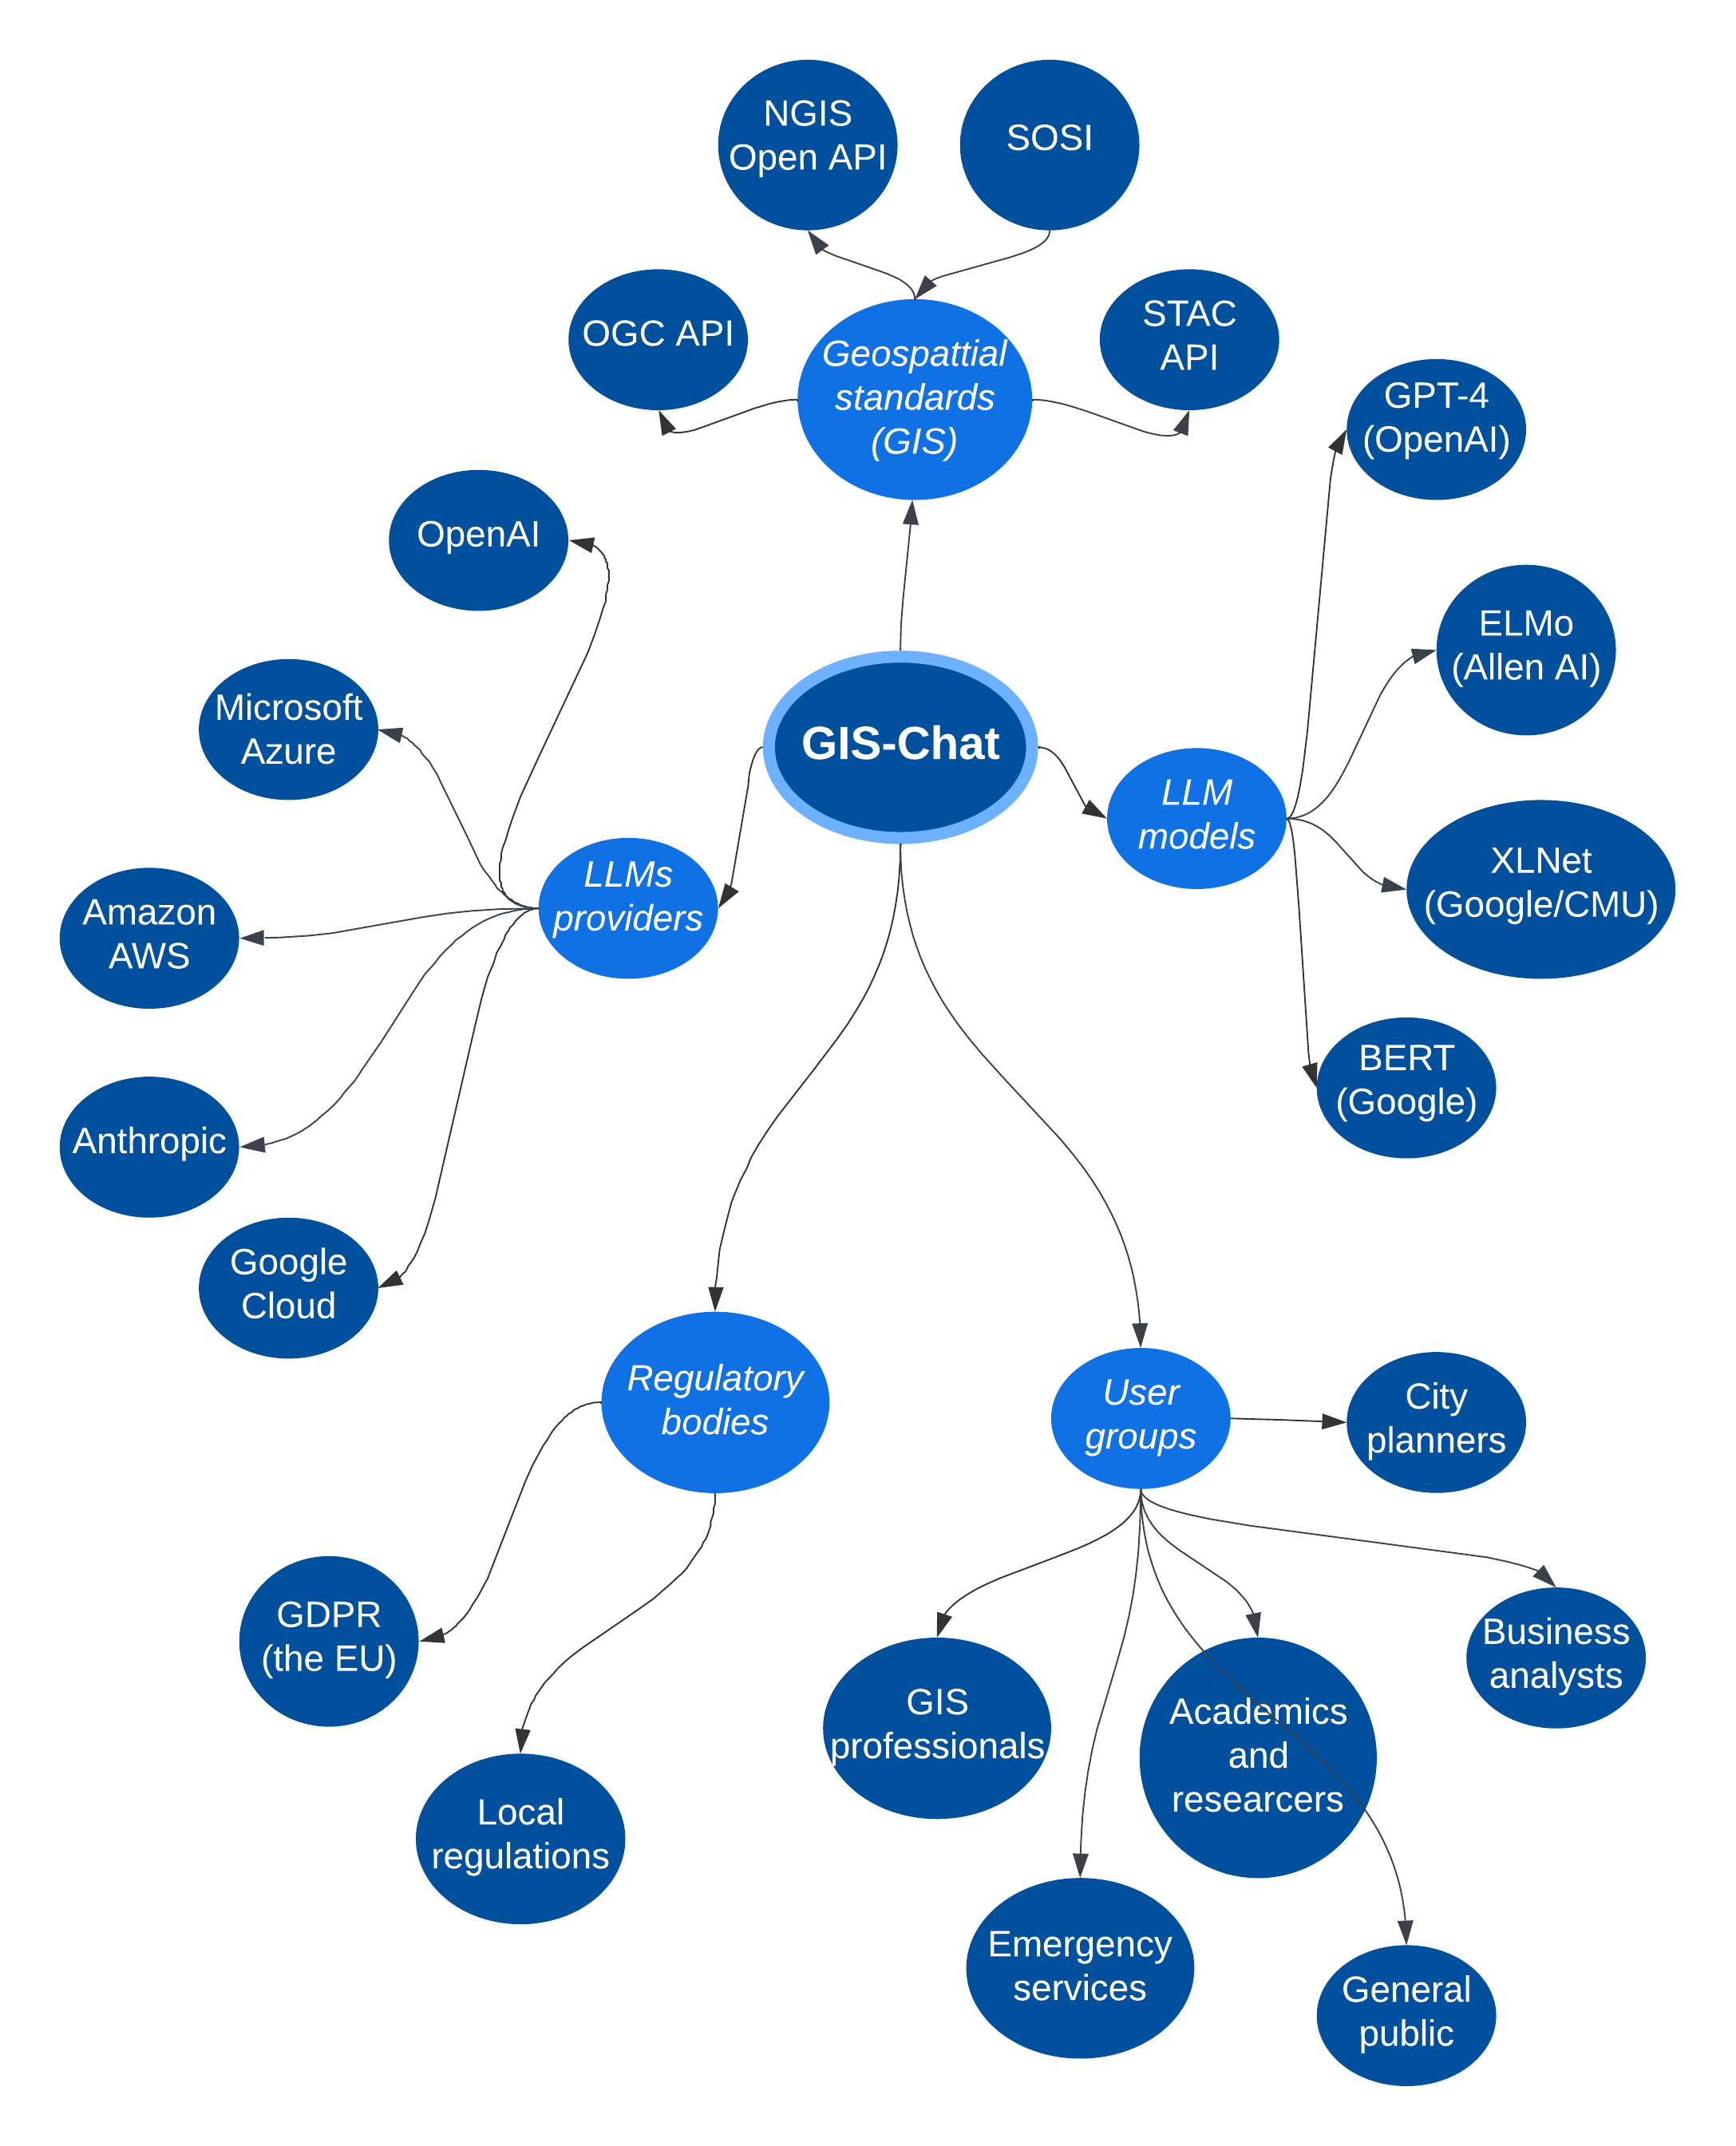
\includegraphics[width=\textwidth]{actor_map}
    \caption{Actor map for stakeholders, providers, and other groups and organizations that could have some relevance to an autonomous LLM-based GIS-agent.}
    \label{fig:actor-map}
\end{figure}

\section[Large Language Models]{\acrlongpl{acr:llm}}\label{sec:llms}

\acrfull{acr:llm} have proved proficient at \gls{acr:nlu} and \gls{acr:nlg}, which are both subfields of \gls{acr:nlp}. \autoref{fig:actor-map} includes six different \acrshortpl{acr:llm} that are all explained in the subsections below. All but the \acrshort{acr:bert} model are made with text generation in mind, with \acrshort{acr:bert} being more adapted for the task of predicting masked tokens, e.g. \enquote{I love going to the \texttt{[MASK]} during summer.}. \acrshort{acr:bert} is very efficient at \gls{acr:nlu}, and is applicable for a range of downstream tasks, one of which is discussed in \autoref{sec:gis-with-llms}. As mentioned, the other \acrshortpl{acr:llm} in \autoref{fig:actor-map} are geared towards text generation, with certain members of the \acrshort{acr:gpt} family and Google's Gemini having multimodal capabilities as well. As \autoref{subsec:social-media} will illustrate, these generative models, known for their great conversational abilities and extensive knowledge from pre-training on large corpora, have been found useful in \gls{acr:gis} analysis. The combination of conversational and visual skills, particularly in multimodal models, holds significant promise for \gls{acr:gis} analysis, where visual interpretation of maps is crucial.

This section will open with an explanation of the fundamental building block of modern \acrlongpl{acr:llm}, namely the Transformer. \Autosubsectionref{subsec:gpt} and \autoref{subsec:bert} will then discuss the two most famous families of \acrshortpl{acr:llm}, namely the \acrshort{acr:gpt}'s and the \acrshort{acr:bert}'s. \Autosubsectionref{subsec:gemini} will present the brand new multimodal Gemini model from Google, and \autoref{subsec:open-source-llms} will list various open-source alternatives.

\subsection{Attention and The Transformer Architecture}\label{subsec:attention-and-transformers}

\cite{vaswaniAttentionAllYou2017} managed to achieve new state-of-the-art results for machine translation tasks with their introduction of the Transformer architecture. The Transformer has later been proved effective for numerous downstream tasks, and for a variety of modalities. Titling their paper \citetitle{vaswaniAttentionAllYou2017}, \citeauthor{vaswaniAttentionAllYou2017} suggest that their attention-based architecture renders network architectures like \glspl{acr:rnn} redundant, due to its superior parallelization abilities and the shorter path between combinations of position input and output sequences, making it easier to learn long-range dependencies \citep[6]{vaswaniAttentionAllYou2017}.

The Transformer employs self-attention, which enables the model to draw connections between arbitrary parts of a given sequence, bypassing the long-range dependency issue commonly found with \glspl{acr:rnn}. An attention function maps a query and a set of key-value pairs to an output, calculating the compatibility between a query and a corresponding key \citep[3]{vaswaniAttentionAllYou2017}. Looking at \citeauthor{vaswaniAttentionAllYou2017}'s proposed attention function \eqref{eq:attention}, we observe that it takes the dot product between the query $Q$ and the keys $K$, where $Q$ is the token that we want to compare all the keys to. Keys similar to $Q$ will get a higher score, i.e., be \textit{more attended to}. These differences in attention are further emphasized by applying the softmax function. The final matrix multiplication with the values $V$, being the initial embeddings of all input tokens, will yield a new embedding in which all individual tokens have some context from all other tokens. We improve the attention mechanism by multiplying queries, keys, and values with weight matrices learned through backpropagation. Self-attention is a special kind of attention in which queries, keys, and values are all the same sequence.

\begin{equation}
    \text{Attention}(Q, K, V) = \text{softmax}\left(\frac{QK^T}{\sqrt{d_k}}\right)V
    \label{eq:attention}
\end{equation}

Attention blocks can be found in three places in the Transformer architecture \citep[5]{vaswaniAttentionAllYou2017} (I will use machine translation from Norwegian to German as an example):

\begin{enumerate}
    \item In the encoder block to perform self-attention on the input sequence (which is in Norwegian)
    \item In the decoder block to perform self-attention on the output sequence (which is in German)
    \item In the decoder block to perform cross-attention (also known as encoder-decoder attention) where each position in the decoder attends to all positions in the encoder
\end{enumerate}

The Transformer represented a breakthrough in the field of \gls{acr:nlp}, and is the fundamental building block of modern \glspl{acr:llm}, most famous of which are the \acrshort{acr:gpt}'s.

\subsection[The GPT Family]{The \acrshort{acr:gpt} Family}\label{subsec:gpt}

\gls{acr:gpt} is a type of \gls{acr:llm} that was introduced by OpenAI in 2018 \citep{radfordImprovingLanguageUnderstanding2018}. Specifically designed for text generation, a \acrshort{acr:gpt} is essentially a stack of Transformer \textit{decoders}, and demonstrates through its vast training on unlabelled data that such unsupervised training can help a language model learn good representations, providing a significant performance boost while alleviating the dependence on supervised learning. While the original Transformer architecture as described by \cite{vaswaniAttentionAllYou2017} was intended for machine translation, thus having encoder to learn the representation of the origin language representation of a given input sequence and an encoder to learn the representation in the target language and perform cross-attention between the two, the \acrshort{acr:gpt} is designed only to \textit{imitate} language. This is why there are no encoders to be found in the \acrshort{acr:gpt} architecture. The model employs masked multi-head attention (running the input sequence through multiple attention heads in parallel), and is restricted to only see the past $k$ tokens---with $k$ being the size of the context window---and is tasked to predict the next one.

Training consists of two stages: unsupervised pre-training and supervised fine-tuning. The former is used to find a good initialization point, essentially teaching the model to imitate the corpora upon which it is trained. This results in a model that will ramble on uncontrollably, just trying to elaborate upon the input sequence it's given to the best of its knowledge. This will naturally produce undefined behaviour, and it is therefore necessary to fine-tune the model on a target task in a supervised manner. \cite[4]{radfordImprovingLanguageUnderstanding2018} explain how the model can be fine-tuned directly on tasks like text classification, but how one for other tasks needs to convert structured inputs into ordered sequences because the pre-trained model was trained on contiguous sequences of text. In the case of ChatGPT, \citeauthor{openaiIntroducingChatGPT2022} used \gls{acr:rlhf} by employing a three-step strategy: first training using a supervised policy, then using trained reward models to rank alternative completions produced by ChatGPT models, before fine-tuning the model using \gls{acr:ppo}, which is a way of training \acrshort{acr:ai} policies. This pipeline is then performed for several iterations until the model produces the desired behaviour \citep{openaiIntroducingChatGPT2022}.

\subsection[The BERT Family]{The \acrshort{acr:bert} Family}\label{subsec:bert}

\gls{acr:bert}, introduced about four months after \cite{radfordImprovingLanguageUnderstanding2018} presented the \acrshort{acr:gpt} architecture, is a family of language models which was first introduced in 2018 and is designed to facilitate a wide range of downstream tasks \citep[5]{devlinBERTPretrainingDeep2019}. The \acrshort{acr:bert} architecture consists of stacked bidirectional Transformer \textit{encoders}. This makes \acrshort{acr:bert} unsuitable for text generation, unlike the \textit{decoder}-based \acrshort{acr:gpt} architecture. However, the self-attention in the encoder, in which tokens can \textit{see} both past and future tokens, mechanism allows for training of deep bidirectional representations, facilitating a wide range of \gls{acr:nlp} tasks. The input sequence is transformed into embeddings (vector representations). These per-token embeddings include information about the meaning of the word itself, the meaning of the sentence/segment it belongs to, and the token's position in the full input. These embeddings then pass through a stack of Transformer encoders (12 and 24 for \textbf{\acrshort{acr:bert}\textsubscript{BASE}} and \textbf{\acrshort{acr:bert}\textsubscript{LARGE}}, respectively), allowing the model to learn more complex patterns, and patterns of different granularities (token, sentence, document) \citep[5]{devlinBERTPretrainingDeep2019}.

The \acrshort{acr:bert} framework consists of two training steps, namely the pre-training and fine-tuning procedures. \acrshort{acr:bert} is pre-trained on two \gls{acr:nlp} tasks. One of these is \gls{acr:mlm}, in which 15\% of words are masked with the special \texttt{[MASK]} token and are left for the model to predict \citep[4]{devlinBERTPretrainingDeep2019}. The \gls{acr:mlm} task helps the model learn bidirectional representations. The second of these unsupervised tasks is \gls{acr:nsp}, where the special \texttt{[CLS]} token (found at the start of each tokenized sequence) is used to predict if a sentence \texttt{B} follows \texttt{A}. During this pre-training step, the input sequence looks like this:

$$
    \texttt{[CLS]} \text{ this is sentence A } \texttt{[SEP]} \text{ and this is sentence B } \texttt{[SEP]}
$$

\noindent The \texttt{[CLS]} token is used to label sentence B as either \texttt{IsNext} or \texttt{NotNext}.

\acrshort{acr:bert} is normally fine-tuned to specific downstream tasks by using the \texttt{[CLS]} token, which captures an aggregated representation of the input sequence. This vector representation can then be used as input to a classification layer for tasks like multi-label classification and regression.

\subsection{Gemini}\label{subsec:gemini}

As of writing, Google's Gemini \citep{geminiteamGeminiFamilyHighly2023}, introduced on December 6th 2023, is the latest addition to the ever-growing pool of \acrlongpl{acr:llm}. Being fundamentally designed for multimodality, it is able to reason between text, images, video, audio, and code. It is being released in three different sizes: the Gemini Ultra, the Gemini Pro, and the Gemini Nano. The Gemini Ultra produces state-of-the-art performance on 30 of 32 widely-used academic benchmarks, and performs worse than \citeauthor{openaiGPT4TechnicalReport2023}'s \acrshort{acr:gpt}-4 on only one benchmark, namely the HellaSwag benchmark for common-sense reasoning for everyday tasks. The Gemini Ultra outperforms \acrshort{acr:gpt}-4 on the \gls{acr:mmlu} benchmark, various reasoning benchmarks, and shows significant improvements in maths and code related benchmarks  \citep[7]{geminiteamGeminiFamilyHighly2023}. Gemini performs better than \citeauthor{openaiGPT4TechnicalReport2023}'s multimodal equivalent in \acrshort{acr:gpt}-4V on all benchmarks \citep[12]{geminiteamGeminiFamilyHighly2023}. Some of these benchmarks are discussed further in \autoref{subsec:benchmarks}.

Like the \acrshort{acr:gpt} architecture, Gemini is built on top of Transformer decoders. Gemini is trained to accommodate various modalities, supporting interleaved sequences of text, image, audio, and video as inputs \citep[3-4]{geminiteamGeminiFamilyHighly2023}. This highlights one of the greatest strengths of the Transformer architecture, namely that it can be adapted for multiple modalities. Commonly, multimodal \acrshort{acr:ai} architectures consist of an ensemble of models, one for each given modality, with different representations that can be difficult to combine. The Transformer solves this issue and provides a common architecture that can be trained end-to-end.

\subsection{Open-Source Alternatives}\label{subsec:open-source-llms}

Seeing as the state-of-the-art models of today, like \acrshort{acr:gpt}-4 and Gemini Ultra, are generally closed-source, it is important to note that there are viable open-source alternatives out there. This section lists the most prominent ones.

\subsubsection[LLaMA]{\acrshort{acr:llama}}

Perhaps the most famous family of open-source \acrshortpl{acr:llm} are Meta AI's \acrshort{acr:llama} (\acrlong{acr:llama}) models, with \acrshort{acr:llama} 2 being the latest addition \citep{touvronLlamaOpenFoundation2023a}. \acrshort{acr:llama} 2 is a powerful family of pre-trained and fine-tuned \acrshortpl{acr:llm} that outperformed open-source chat models on most benchmarks at its release. It also shows great results in terms of safety, even outperforming the closed-source ChatGPT-0301 model. The training process of \acrshortpl{acr:llama} is similar to that of the \acrshort{acr:gpt} model, with pre-training being performed using an optimized auto-regressive transformer which is trained from a large corpus of unstructured data. \acrshort{acr:llama} is then fine-tuned using various alignment techniques, and the authors also share a new technique called Ghost Attention, which aims to control dialogue flow over multiple turns. \gls{acr:rlhf} and \gls{acr:ppo} are other important techniques used to get the desired behaviour out of the model.

Many flavours of \acrshort{acr:llama} have been trained. Most notably is Code \acrshort{acr:llama} 2 \citep{roziereCodeLlamaOpen2023}, a family of \acrshortpl{acr:llm} fine-tuned for code, scoring at 53\% and 55\% on the HumanEval and \gls{acr:mbpp} benchmarks, respectively. Vicuna-13B is another example of a \acrshort{acr:llama}-based model, and is fine-tuned on user-shared conversations collected from ShareGPT\footnote{\url{https://sharegpt.com/}}, a website where users can upload ChatGPT conversations. At its release in March 2023, it achieves more than 90\% quality of OpenAI's ChatGPT and Google's Bard, while also outperforming the original \acrshort{acr:llama} model.

\subsubsection{Mistral}

Mistral 7B \citep{mistralaiMistral7B2023} is another open-source \acrshort{acr:llm}, and is claimed by its creators at Mistral \acrshort{acr:ai} to be \enquote{the most powerful language model for its size to date}. Being a 7.3B parameter model, it is quite small compared to other models, such as the 1.76T parameter \acrshort{acr:gpt}-4 model. Mistral 7B outperforms the \acrshort{acr:llama} 2 13B on all benchmarks, and approaches Code \acrshort{acr:llama} 7B performance on code.

\subsubsection{Orca 2}

Orca 2 \citep{mitraOrcaTeachingSmall2023}, developed at Microsoft, is an open-source \acrshort{acr:llm} with exceptional step-by-step reasoning capabilities. It is based on \acrshort{acr:llama} 2 and is fine-tuned on curated training data from a more capable teacher model like \acrshort{acr:gpt}-4. Evaluation results shows that the Orca-2-13B model surpasses models of the same size, and that it is competitive with models 5-10x larger, exceeding the performance of \acrshort{acr:llama}-2-Chat70B and performing comparably to ChatGPT on reasoning tasks \citep[11-12]{mitraOrcaTeachingSmall2023}. It does have some limitations, most notably in terms of potential of misuse due to the lack of suitable safeguards like \gls{acr:rlhf} training \citep[21]{mitraOrcaTeachingSmall2023}.



\section[LLM providers]{\acrlong{acr:llm} Providers}\label{sec:llm-providers}

The \acrshort{acr:ai} community called Hugging Face\footnote{\url{https://huggingface.co/}} is the most widely used hub for open-source and open-science machine learning. It is used by both individual community members and large commercial actors like Google Cloud and Meta \acrshort{acr:ai} as a way of contributing to the world open-source \acrshort{acr:ai}. Hugging Face's \texttt{transformers} Python library\footnote{\url{https://github.com/huggingface/transformers}} provides an interface with their hub, which at the time of writing has 177k stars on GitHub.

OpenAI is one of the leading providers of \acrshortpl{acr:llm}, most prominently through their \acrshort{acr:gpt} series. While originally founded as an open-source company, their models are now closed-source and their \acrshort{acr:gpt} \acrshortpl{acr:api} are paid services. It should be noted, however, that they still are great contributors to open-source having uploaded a range of speech detection and diffusion models to Hugging Face.

Microsoft Azure, the main partner of OpenAI, provides \acrshortpl{acr:api} for OpenAI's language models including the \acrshort{acr:gpt}-4, \acrshort{acr:gpt}-3.5-Turbo and Embeddings model series. Unlike OpenAI's own \acrshortpl{acr:api}, Microsoft Azure also offers private networking, regional availability, and responsible \acrshort{acr:ai} content filtering\footnote{\url{https://learn.microsoft.com/en-us/azure/ai-services/openai/overview?source=recommendations}}. Also, by using Microsoft Azure's \acrshort{acr:api}, \acrshort{acr:llm} inputs and outputs are unavailable to OpenAI, which is not the case otherwise\footnote{\url{https://learn.microsoft.com/en-us/legal/cognitive-services/openai/data-privacy}}.

\cite{clearyLatencyBenchmarksComparisons2023} did benchmarking of different \acrshortpl{acr:llm} on different providers. Important takeaways were that \acrshort{acr:gpt}-4 is about 6.3 times slower than \acrshort{acr:gpt}-3.5-Instruct, and that Microsoft Azure has far lower latency in most cases for inference on \acrshort{acr:gpt} models compared to OpenAI's own \acrshortpl{acr:api}. Such considerations are important when addressing usability of \acrshort{acr:llm}-based applications, balancing accuracy against speed and cost.

Aforementioned Google Cloud is another large \acrshort{acr:llm} provider. They provide a wide range of services, among these the Vertex \acrshort{acr:ai} platform\footnote{\url{https://cloud.google.com/vertex-ai/}}. Vertex \acrshort{acr:ai} provides \acrshort{acr:api} access to foundational models through their Model Garden platform which supports first-party, open-source, and third-party models. Vertex \acrshort{acr:ai} also provides experimental prompt design and fine-tuning services. Vertex \acrshort{acr:ai} is a paid service.

Anthropic\footnote{\url{https://www.anthropic.com/}} is another closed-source \acrshort{acr:llm} provider that has grown rapidly in size since their launch in 2021, and focus on creating safer, steerable, and more reliable models. Their flagship model is Claude 2.1, which has a large context window of 200,000 tokens, enabling users to upload large technical documentation that the model can keep in its memory when creating responses. Anthropic lists complex reasoning, creativity, and coding as Claude's major strengths.

There are numerous open-source alternatives to the closed-source resources. Using free open-source alternatives where possible is a good option to reduce cost. Meta \acrshort{acr:ai}\footnote{\url{https://ai.meta.com/}} is a big contributor to open-source \acrshort{acr:ai}, most famously through Pytorch---a popular deep learning framework---and their LLaMA models (see \autoref{subsec:open-source-llms}). Eleuther \acrshort{acr:ai}\footnote{\url{https://www.eleuther.ai/}} is an open-source centred company with aim to \enquote{increase transparency and reduce potential harms from emerging \acrshort{acr:ai} technologies}. As such, they have released a range of trained \acrshortpl{acr:llm} along with the codebases used to train these. Perhaps most famous is their \acrshort{acr:gpt}-J model, which is an auto-regressive model in the style of \acrshort{acr:gpt}-3, aimed at the English language.

\section{Geospatial Standards}\label{sec:geospatial-standards}

It is important for \acrshort{acr:gis} applications of any kind to support modern geospatial standards. Subsections \ref{subsec:standardization-international} and \ref{subsec:standardization-norway} will provide a brief overview of the standardization work that has been and is being done on the international scene and in Norway, respectively.

\subsection{International Standardization Work}\label{subsec:standardization-international}

International geospatial standardization involves the global collaboration and development of uniform standards and protocols for geospatial data and technologies. The \acrshort{acr:ogc} standards and the \acrshort{acr:stac} \acrshort{acr:api} standard are examples of such work.

\subsubsection[OGC Standards]{\acrshort{acr:ogc} Api Standard}\label{subsubsec:ogc}

The \gls{acr:ogc} \acrshort{acr:api} standards serve as the glue in the field of \gls{acr:gis}, paving the way for interoperability and data exchange between diverse systems. Leveraging common web protocols like \acrshort{acr:html} and supporting multiple data formats including \acrshort{acr:json}, \acrshort{acr:gml}, and \acrshort{acr:html}, the \gls{acr:ogc} \acrshort{acr:api} standard provides a modular architecture consisting of a core specification and various extensions. According to their webpages, they provide 80 different standards, each for a specific geospatial purpose. Notable examples are 3D Tiles, CityGML, GeoTiff, and \acrshort{acr:ogc} \acrshort{acr:api} - Features \citep{ogcOGCStandards2023}. The \acrshort{acr:ogc} \acrshort{acr:api} standards function as modern replacements to older standards like \acrshort{acr:wms} and \acrshort{acr:wfs}, and presents a more adaptable framework for spatial data operations, facilitating innovation in the \acrshort{acr:gis} domain.

\subsubsection[STAC Api Standard]{\acrshort{acr:stac} Api Standard}\label{subsubsec:stac}

The \gls{acr:stac} \acrshort{acr:api} is a standardized way to expose collections of spatial temporal data for online search and discovery. Built upon a \acrshort{acr:json} core, it aims to be a uniform and flexible environment from which developers can customize the API infrastructure to their domain. \acrshort{acr:stac} is closely related to \acrshort{acr:ogc}, and \acrshort{acr:ogc} board member Chris Holmes said in a blog post that \enquote{The \acrshort{acr:stac} \acrshort{acr:api} implements and extends the \gls{acr:ogc} \acrshort{acr:api} - Features standard, and our shared goal is for \gls{acr:stac} \acrshort{acr:api} to become a full \gls{acr:ogc} standard.} \citep{holmesSpatioTemporalAssetCatalogs2021}. \gls{acr:stac} \acrshort{acr:api} provides a powerful query language that allows users to search by various parameters like time, location, and keywords, making it widely applicable. The \acrshort{acr:stac} community has also defined specifications in order remove the complexity associated with having to create unique pipelines when consuming different spatial-temporary collections. The significance of the \gls{acr:stac} \acrshort{acr:api} lies in its ability to democratize access to large volumes of geospatial data. By offering a common standard for data cataloguing and discovery, it reduces the barriers that often exist due to incompatible data formats. Developers or \acrshort{acr:gis} professionals can take advantage of this through built-in tooling in QGIS---a desktop \gls{acr:gis} for viewing, editing, and analysing spatial data---or through third-party packages in the Python and R programming languages. The API is also accessible through the command line interface when using \acrshort{acr:gdal} \citep{STACTutorials}.

\subsection{Norwegian Standardization Work}\label{subsec:standardization-norway}

Geospatial standardization work has been on the agenda of Norwegian governing powers for decades and have materialized in frameworks/collaborations like \nameref{subsubsec:geovekst} and \nameref{subsubsec:norge-digitalt}, as wells as the \nameref{subsubsec:sosi} file format. This standardization work will be the topic of this section.

\subsubsection[SOSI]{\acrshort{acr:sosi}}\label{subsubsec:sosi}

\gls{acr:sosi} is a Norwegian file format for storing and exchanging geospatial data. It was first introduced in 1987 and has since approached international standards, the most important arenas currently being \acrshort{acr:iso}/\acrshort{acr:tc} 211 and \gls{acr:ogc} \citep{mardalNasjonalStrategiVidereutvikling2015}. \gls{acr:sosi} is the adopted Norwegian standard for creating and delivering digital geographic data, administered by the Norwegian Mapping Authority \citep{maehlumSOSI2023}.

In a \gls{acr:sosi} dataset, terrain points, lines, and polygons are represented by their coordinates and classified into various object types according to the \gls{acr:sosi} object catalogue standard. However, there are few GIS systems that can read \gls{acr:sosi} data directly, so data in \gls{acr:sosi} format usually needs to be converted to another \gls{acr:gis}-readable data format \citep{maehlumSOSI2023}.

\subsubsection{Geovekst}\label{subsubsec:geovekst}

Geovekst is a Norwegian initiative that aims for collaborative collection, distribution, management, and maintenance of geospatial information. It was established in 1992, and is a partnership between national, regional, and local government bodies, as well as several private companies.\footnote{\url{https://www.kartverket.no/geodataarbeid/geovekst}} The primary goal associated with Geovekst is to \enquote{collaborate to secure updated Geovekst data to help solve parts of the parties' societal missions} \citep[5]{thenorwegianmappingauthorityHandbokGeovekstsamarbeidet2023}. The objective of the collaboration is to ensure that geographical data is collected \textit{once}, conforming  to \textit{one} standard, maintained in \textit{one} place, and used by \textit{many}. Responsibilities and costs are shared among the parties of the collaboration.

The most important contribution of Geovekst is \gls{acr:fkb}, a series of very detailed Norwegian mapping datasets, serving as rich resources for both public and private sectors. The datasets are obtained through a variety of data sources, including aerial photographs, laser scans, and manual mapping. Geovekst also provides airborne surveys in emergency situations, when the speed of surveying is important.\footnote{\url{https://www.kartverket.no/geodataarbeid/geovekst/datafangst-i-krise}}

\subsubsection[The National Spatial Data Infrastructure]{The \acrlong{acr:nsdi}}\label{subsubsec:norge-digitalt}

Established in 2005, the \gls{acr:nsdi} is a more recent framework compared to Geovekst, and is more often referred to by its Norwegian name: \textit{Norge Digitalt}. The \gls{acr:nsdi} involves governmental bodies (national, regional, and municipal), but also educational and research institutions and companies with responsibilities on a nation-wide scale; examples include Telenor and local and regional energy companies \citep[6]{norgedigitaltGenerelleVilkarNorge2023}. The \gls{acr:nsdi} infrastructure is the sum of common standards and rules, geographical data and services related to these, in addition to tools and deals. It aims to coordinate geospatial activities in Norway, making it easier to discover, access, and use spatial data. The framework is coordinated by the Norwegian Mapping Society \citep{norgedigitaltGenerelleVilkarNorge2023}.



\section{User Groups}\label{sec:user-groups}

There are several user groups that could take advantage of an \acrshort{acr:llm}-based agent with extensive geographic and \acrshort{acr:gis} knowledge. Queries to such an agent could span from simple retrieval questions like \enquote{How many people live in Trondheim} and \enquote{What is Sweden's third largest city?}, to more complicated questions that require problem-solving abilities and reasoning. While it is difficult to obtain good datasets of common queries, \cite{kumarWhatArePeople2023a}---creater of the chatbot app Pocket AI\footnote{\url{https://github.com/varunon9/pocket-ai}}---shared a dataset of \textasciitilde 13k user queries from his app along with classifications of these. Salient categories are listed in \autoref{tbl:query-category-distribution}. The main takeaway from these numbers is that the main motivation for use is productivity.

\begin{table}[ht]
    \centering
    \begin{tabular}{l|c}
        \toprule
        \textbf{Category}                    & \textbf{Percentage} \\
        \midrule
        Task oriented                        & 23.1\%              \\
        Informational                        & 20.2\%              \\
        Social                               & 16.2\%              \\
        Personal advice and self-improvement & 13.1\%              \\
        \bottomrule
    \end{tabular}
    \caption{Distribution of query categories}
    \label{tbl:query-category-distribution}
\end{table}


This aligns with the results of \cite{skjuveWhyPeopleUse2023} from their questionnaire-based study performed in late January 2023, about two months after the release of ChatGPT. The goal with the study was to figure out why people use ChatGPT. They found that most participants (55\%) are motivated by productivity, specifically applying it for routine tasks, information retrieval, text generation and writing support, and software development \citep[17-21]{skjuveWhyPeopleUse2023}. \autoref{tbl:chatgpt-motivation-survey-restuls} shows all categories and their frequencies. There were 197 samples in total, and more than one category could be  assigned to each sample. It is worth noting that the study is likely to have included early adopters, and might therefore make the results less representative for the time at which this report is written (\today), now that use patterns have become more established \citep[37]{skjuveWhyPeopleUse2023}.

\begin{table}[ht]
    \centering
    \begin{tabular}[t]{l|c}
        \toprule
        \textbf{Category}              & \% \textbf{(n)} \\
        \midrule
        Productivity                   & 55\% (109)      \\
        Novelty                        & 51\% (101)      \\
        Fun and amusement              & 20\% (41)       \\
        Creative work                  & 18\% (34)       \\
        Social interaction and support & 9\% (18)        \\
        Other                          & 7\% (15)        \\
        \bottomrule
    \end{tabular}
    \caption{Categories and frequency of ChapGPT usage \citep[16-17]{skjuveWhyPeopleUse2023}.}
    \label{tbl:chatgpt-motivation-survey-restuls}
\end{table}

The main reason people use conversational \acrshort{acr:ai} is thus for productivity, whether in a professional, academic, or personal context. 67 out of the 197 participants in \cite[18]{skjuveWhyPeopleUse2023} highlighted ChatGPT's ability to understand complex queries and that it is "efficient in alleviating the need to experiment with different phrasings of the query", as is often needed when 'Googling' for an answer to a specific question. The ease of information retrieval, along with it's problem-solving abilities \citep[20]{skjuveWhyPeopleUse2023}, could also make conversational \acrshortpl{acr:ai} highly relevant for \acrshort{acr:gis}-related purposes.

One could imagine a range of potential user groups that could benefit from such an artificial, and spatially aware, companion. Some suggested user groups are presented in \autoref{fig:actor-map}. Perhaps the most obvious one is that of the \acrshort{acr:gis} professionals. While an \acrshort{acr:ai}-based \acrshort{acr:gis} agent more capable than the average \acrshort{acr:gis} professional is currently far from becoming a reality, such an agent could help suggest strategies of solving a particular problem using the input data available and a good user prompt, or it could help solve mundane tasks in an automated way in order to allow \acrshort{acr:gis} professionals to allocate more time to creative and complex tasks.

Closely related to \acrshort{acr:gis} professionals are the city planners. Though often less knowledgeable in the field of \acrshort{acr:gis}, they are increasingly dependent upon geospatial analysis in order to make informed decisions. Having an easy-to-use \acrshort{acr:gis} ready at any moment could prove both time- and -cost-saving. The same goes for business analysts and people involved in academia. The \textit{time} variable is especially important to the emergency services. At the impact of a natural disaster like a flood or forest fire, geospatial analysis could prove lifesaving. Having powerful geospatial knowledge even in the absence of a \acrshort{acr:gis} professional is therefore important in order to focus resources to areas where the situation is most pressing.

An \acrshort{acr:llm}-based agent with geospatial awareness could also be useful to the general public; one may want to find suitable biking routes or good hills to do interval running in, or to know what areas are prone to flooding when buying a house. Most people do not possess the knowledge or time to perform such analyses themselves, so an automated \acrshort{acr:ai}-based agent could prove useful for such use cases.



\section{Ethical and Privacy Concerns}\label{sec:ethical-and-privacy-concerns}

Although an \acrshort{acr:ai}-based \acrshort{acr:gis} agent could prove powerful, there are some ethical pitfalls in terms of regulations and privacy concerns that need consideration. If such an agent is to make decision on behalf of humans it is important that one can hold someone accountable in the case that something goes wrong. If an \acrshort{acr:ai}-based agent is tasked to lead firefighters to the tactically optimal locations in order to quench a fire, but  instead misleads them and traps them inside the fire, who is then to blame? \cite{sparrowKillerRobots2007} provides an interesting angle on such issues, though in his essay related the role of artificially intelligent robots in modern warfare.

Furthermore, it is vital to ensure that the \acrshort{acr:ai} agent is not utilized for immoral purposes, like finding the optimal location in which to dissolve poison into people's drinking water to maximize the number of people killed. Work has been done with newer \acrshortpl{acr:llm} to prevent them from producing dangerous, misinformed, or toxic text---this issue is widely discussed in the technical report of the latest \acrshort{acr:gpt} model \citep[11-14]{openaiGPT4TechnicalReport2023}---but there have been cases where these issues haven't been considered well enough.\footnote{The \acrshort{acr:llama}-based Alpaca model, developed at Stanford University, was taken offline after being shown to produce misinformation, toxic text: \url{https://www.theregister.com/2023/03/21/stanford_ai_alpaca_taken_offline/}}

The \gls{acr:gdpr} entered into applicability in the European Union in 25th of May 2018, and although not a member of the European Union, Norway incorporated the \gls{acr:gdpr} in July the same year due to its membership of the European Economic Area. The \gls{acr:gdpr} imposes stricter regulations about data privacy, meaning people have more control over their personal data, and that businesses get a level playing field in terms of what customer information is available \citep{datatilsynetGeneralDataProtection}. With data privacy arguably being more relevant thanever, we must make certain that \acrshort{acr:ai}-based \acrshort{acr:gis} agents are unable to access and spread information of private or sensitive character, even if such information has become publicly available by accident---as was the case when the Norwegian Broadcasting Corporation (NRK) was able to (legally) obtain accuracy geolocations of central people in the Norwegian army from a commercial London-based company\footnote{Link to news article in Norwegian: \url{https://www.nrk.no/norge/xl/norske-offiserer-og-soldater-avslort-av-mobilen-1.14890424}}.

\glsresetall
\chapter{Related Work}
\label{cha:related-work}

\begin{comment}
What other research has been conducted in this area and how is it related to your work?
This section is thus where your literature review will be presented. It is important when presenting the review
that you give an overview of the motivating elements of the work going on in your field and how these relate to your work,
rather than a list of contributors and what they have done.
This means that you need to extract the key important factors for your work and discuss how others have addressed
each of these factors and what the advantages/disadvantages are with such approaches.
As you mention other authors, you should reference their work.
Note that the reference list reflects the literature you have read {\em and\/} have cited.
This will only be a subset of the literature that you have read.

A good way to find relevant work is by checking what others are referencing, e.g., in papers you have already found
However, when doing that,
do not fall into one of the common traps, such as re-iterating someone's false quote or faulty analysis of
a previous paper (check the original source!), or getting stuck inside a local research cluster (a group of
researchers that mainly refer to the ones using the same type of approaches or similar ideas).

Make sure that it is clear how and why you decided to include some references (and discard others). As in all parts of research, it should ideally be possible for someone else to reproduce your work, also when it comes to finding the relevant references.
There are (at least) three basic methods for finding references:
\begin{enumerate}
    \item Trust the authorities (e.g., your supervisor) to dig out good texts for you.
          Those can often be used as a seed set for:
    \item Snowballing, where you have some good articles and check the references in them for other good ones.
          Note that this can be done both backwards and forwards on the timeline; that is, using tools like Google Scholar, you can also check who refers \textit{to\/} the good articles you have already found.
\end{enumerate}

Note that a reference needs to be complete: you should always give the full name of a conference or journal,
always include page numbers, always say where a book or thesis was published, and where a conference took place, as further described in Section~\ref{sec:reference_list}.
\end{comment}

The related works are divided into three sections, each being relevant to the project in different ways. \Autosectionref{sec:gis-with-llms} is the most obviously relevant section, discussing works in which \acrshortpl{acr:llm} were employed to perform tasks in the geospatial realm. \Autosectionref{sec:prompt-engineering-and-planning-strategies} delves into different prompt engineering and planning strategies that could be useful to make an autonomous \acrshort{acr:gis} agent perform better and more reliably. \Autosectionref{sec:retrieval-automented-generation} discusses \gls{acr:rag}, that is, how one can provide an autonomous \acrshort{acr:llm}-based agent with externaFcontributionsl tooling and up-to-date information. \cite{wengLLMPoweredAutonomous2023} provides a good summary of techniques relevant to \autoref{sec:prompt-engineering-and-planning-strategies} and \autoref{sec:retrieval-automented-generation}.



\section[GIS with LLMs]{\acrshort{acr:gis} with \acrshortpl{acr:llm}}\label{sec:gis-with-llms}

A substantial body of work have been done in recent years to assess the geospatial knowledge of \acrshortpl{acr:llm}, and how they can be fine-tuned or embedded into frameworks to serve downstream tasks.

\subsection{Taking the Temperature on GIS with LLMs on Social Media}\label{subsec:social-media}

The search term \enquote{LLM GIS} on Twitter/X shows various ways that people are using \acrshortpl{acr:llm} for \acrshort{acr:gis}-related tasks. One user praises the use of ChatGPT to \enquote{extract and categorize data from unstructured text}, sharing a video from an ESRI conference\footnote{\url{https://twitter.com/mildthing99/status/1658507921234296833}}. Twitter user Zeke Hausfather shares the discovery that \enquote{\acrshort{acr:gpt}4 now supports processing netCDF files and other geospatial data, as well as some pretty amazing visualization}\footnote{\url{https://twitter.com/mildthing99/status/1658507921234296833}}. Arpit Gupta shares a summary of a paper on generative regulatory measurement on Twitter/X, where he explains how they have utilized \acrshortpl{acr:llm} to decode and interpret status updates and administrative documents, including, for instance, mapping zoning and housing regulations for the suburbs of Chicago\footnote{\url{https://twitter.com/arpitrage/status/1723033894801309893}}. Yu Zhao speculate in the effectiveness of smaller \acrshortpl{acr:llm} fine-tuned on domain-specific knowledge for \acrshort{acr:gis} or remote sensing\footnote{\url{https://twitter.com/zhaoyutim/status/1651233975946321920}}, an interest other users share\footnote{\url{https://twitter.com/zhaoyutim/status/1651233975946321920}}\footnote{\url{https://twitter.com/DougButdorf/status/1670938318979121152}}.

Swapping out \enquote{LLM} with \enquote{ChatGPT} gave more results. One user shows you using ChatGPT with tabular geographical data can increase productivity\footnote{\url{https://twitter.com/BooneLovesVideo/status/1617479222724857856}}. Other users show how they use ChatGPT for entertainment  or as an educational tool in a \acrshort{acr:gis} context\footnote{\url{https://twitter.com/briankingery87/status/1631365717269307394}}\footnote{\url{https://twitter.com/burdGIS/status/1614630141858316288}}\footnote{\url{https://twitter.com/_jsolly/status/1652867118797590528}}\footnote{\url{https://twitter.com/wanjohikibui/status/1628282272548806657}}\footnote{\url{https://twitter.com/GeoWithJustin/status/1641155652759199744}}. This appears to be the primary method by which people utilize ChatGPT, and it seems to offer mostly adequate responses. Another user highlights ChatGPT's built-in geographical context, using it to get GeoJSON polygons for a specified are directly\footnote{\url{https://twitter.com/at_dot_Py/status/1649985754800730112/}}.

On YouTube, the search term \enquote{ChatGPT GIS} yield a range of relevant responses. Several videos display how ChatGPT can be used to create Python code for \acrshort{acr:gis}-related purposes. Examples were found of users highlighting ChatGPT's abilities to generate Python code to manipulate geospatial files, perform analysis, and visualize, using Python libraries like GeoPandas and Folium\footnote{\url{https://www.youtube.com/watch?v=QDf-zc81NSE&t=1707s&ab_channel=GeoDeltaLabs}}\footnote{\url{https://www.youtube.com/watch?v=iNHQgLw7qZc&ab_channel=GeoDeltaLabs}}\footnote{\url{https://www.youtube.com/watch?v=BK2IzZZZC-k&ab_channel=MattForrest}}. Other users show how uploading geospatial files into ChatGPT using Code Interpreter can be an efficient workflow\footnote{\url{https://www.youtube.com/watch?v=dgzWLBYswh0&ab_channel=MiningGeologist}}. Some user demonstrate the QChatGPT\footnote{\url{https://plugins.qgis.org/plugins/QChatGPT/}} plugin to QGIS, which is a plugin integration between QGIS and the OpenAI \acrshort{acr:api}. QChatGPT does not seem to have any context of the current QGIS project the user is working on, but appears to have sparked some excitement among certain users, seeing how \acrshortpl{acr:llm} can assist them in their daily work as \acrshort{acr:gis} professionals\footnote{\url{https://www.youtube.com/watch?v=zUZs4GsDk6I&ab_channel=GISWorld}}\footnote{\url{https://www.youtube.com/watch?v=eEkVTUS8Qtc&ab_channel=HansvanderKwast}}\footnote{\url{https://www.youtube.com/watch?v=Tc-hHaDqoxY&ab_channel=DEVICKSGEOSPATIALCO.}}. One user shows an application with ChatGPT integration that can generate \acrshort{acr:sql} code and visualize geospatial data\footnote{\url{https://www.youtube.com/watch?v=gaA46aaWDuc&ab_channel=GeospatialWorld}}. A recurring user shows how one can use LangChain and its \acrshort{acr:sql} database plugins to \enquote{unlock ChatGPT's potential}\footnote{\url{https://www.youtube.com/watch?v=FoGm7d0paIo&t=1190s&ab_channel=MattForrest}}.

Lastly, the \enquote{FME Channel} released a recording of a webinar where they show how \acrshort{acr:gpt}-3 is being used in FME Data Integration Workflows\footnote{\url{https://www.youtube.com/watch?v=94ZDhgW8yMY&ab_channel=FMEChannel}}. They highlight how the OpenAI \acrshort{acr:api} allows for easy and automated no-code \acrshort{acr:api} to \acrshort{acr:api} workflows. On the FME Community website, an article writes about the \texttt{OpenAICompletionsConnector} and \texttt{OpenAIImageGenerator} transformers in FME\footnote{\url{https://community.safe.com/s/article/Tutorial-Getting-Started-with-OpenAI-in-FME}}. They list use cases such as, running data through the \acrshort{acr:ai} for analysis, generation of reports and summaries, generating scripts or \acrshort{acr:sql} for use in a data integration workflow, and automatic generation of images based on a dynamic input.



\subsection[Geospatial Context in LLMs]{Geospatial Context in \acrshortpl{acr:llm}}

\cite{scherrerHeLjuVarDial20202020} were able to show that \acrshort{acr:bert} can be fine-tuned to accurately predict geolocations from textual input, by winning a shared task on predicting geolocations from Twitter/Jodel messages in a workshop in 2020 \citep{gamanReportVarDialEvaluation2020}. By converting the task into a double regression problem, where they predicted latitude/longitude pairs from the output \texttt{[CLS]} representation of \acrshort{acr:bert} models. For a subtask on a Swiss Jodel dataset, they were able to achieve a median distance of 15.72 km from the ground truth, showing that \acrshortpl{acr:llm} can be trained correlate lingual features and geolocations.

\cite{robertsGPT4GEOHowLanguage2023} investigated extent of GPT-4's geospatial awareness through a set of case studies with increasing difficulties, starting with general factual tasks and finishing with complex questions such as generating country outlines and travel networks. The authors find that \acrshort{acr:gpt}-4 is \enquote{skilful at solving a variety of application-centric tasks}, almost having the ability to \enquote{see}, despite being a language model and thus only being able to interface with the world through sequenced, textual input. Examples include its ability to perform as a travel assistant in providing itinerary suggestions for a trip when provided with requirements, and its ability to provide start and end locations bird migrations generally correct, and in some cases highly accurate. While it becomes obvious that a lot of geospatial context have been embedded within the model during the vast pre-training, the question whether this is memorization or reasoning is a central one. The authors suggest that variability of tasks in their experiments deems it unlikely that it is all memorization, but they say that some things appear to be memorized.

\cite{mooneyUnderstandingGeospatialSkills2023} examined the performance of ChatGPT in a \acrfull{acr:gis} exam, aiming to assess its ability to grasp various geospatial concepts, highlighting its capabilities and limitations. Experiments were conducted on GPT-3.5 and GPT-4, which delivered performances equivalent to grades of D and B+, respectively. Additional experiments were conducted for more specialized areas of \acrshort{acr:gis}, including True/False questions about spatial analysis, and simple tasks in applied \acrshort{acr:gis} workflow. Experiments on the latter showed that ChatGPT-4 was able to correctly answer a relatively complex \acrshort{acr:gis} tasks involving seven different datasets, requiring seven steps in order to obtain a perfect score. Generally, ChatGPT-4 outperformed ChatGPT-3.5 in all tasks. While clearly powerful, the authors highlight a range of limitations, among which the multimodal nature of \acrshort{acr:gis}, which would hinder a straightforward application of existing models.

\cite{unluChatmapLargeLanguage2023} discussed importance of enabling \acrshortpl{acr:llm} to recognize and interpret geospatial data, and how \gls{acr:osm} can play an important role in offering \acrshortpl{acr:llm} linguistic access to vast cartographic datasets. He exemplifies this claim through a proof of concept in which he performs small-scale fine-tuning on an \acrshort{acr:llm} with 1B parameters, using an artificial supervised datasets curated by the more capable ChatGPT 3.5-turbo, which functions as a teacher model, generating prompt-answer pairs for given preprompts. The fine-tuned model displays promising ability of answer questions about a location's attributes, allowing the user to inquire about things like tourist appeal and potential profitability of businesses in the vicinity of the given location. \citeauthor{unluChatmapLargeLanguage2023} emphasizes the method's strengths for small datasets and minimal computational settings. The study also investigated the idea of using embeddings of the curated prepromts. Experimenting with average GLOVE embeddings, he showed that the latent structure of verbal descriptions of \gls{acr:osm} data can yield insightful patters. This, he argues, can prove useful when creating \acrfull{acr:rag} applications aimed at allowing users to retrieve geospatial information in a prompt-based manner.

\subsection[Autonomous GIS]{Autonomous \acrshort{acr:gis}}

\cite{liAutonomousGISNextgeneration2023} states that “autonomous \acrshort{acr:gis} will need to achieve five autonomous goals: self-generating, self-organizing, self-verifying, self-executing, and self-growing.”, and provide a “divide-and-conquer”-based method to address some of these goals. Furthermore, they propose a simple trial-and-error approach to addressing the self-verifying goal. They also highlight need of a memory system in a mature \gls{acr:llm}-based \gls{acr:gis} system, referring to the use of vector databases in autonomous agents like AutoGPT \citep{richardAutoGPTHeartOpensource2023}. Even with its shortages, the solution that \citep{liAutonomousGISNextgeneration2023} provide, called \acrshort{acr:llm}-Geo, is able to solve provide good solutions in various case studies by providing executable assemblies in a Python environment when provided with URLs to relevant data sets, along with a user-specified query.

\cite{zhangGeoGPTUnderstandingProcessing2023} use the LangChain framework \citep{chaseLangChain2022} in order to combine different GIS tools in a sequence in order to solve different sub-goals, and focuses on using the semantic understanding and reasoning abilities of \glspl{acr:llm} like (e.g., ChatGPT) to call externally defined tools, employing the \gls{acr:llm} as an agent or controller. The authors take great inspiration from the AutoGPT framework \citep{richardAutoGPTHeartOpensource2023}. The externally defined tools are described (manually) by its name and description. Said description contains information about the input parameters and output types of the tools/functions. Tools are defined for geospatial data collection, data processing and analysis, and data visualization. The effectiveness of the system is showcased in four case studies.

\cite{qiMaaSDBSpatialDatabases2023} discuss how \acrshortpl{acr:llm} can be used in spatial data management, facilitating a system that can learn from both structured and unstructured data, the latter of which is possibly the greatest strength of modern \acrshortpl{acr:llm}. They highlight the opportunity that \acrshortpl{acr:llm} provide in reducing the barrier to information retrieval for the general public, and discuss how these strengths can be used in spatial data management by leveraging a spatial database system trained from both structured and unstructured data, allowing for seamless access to spatial knowledge, also for those with little or no expertise in querying a spatial database. With that in mind, they envisage to use \textit{machine learning models as a spatial database} (MaaSDB), which when trained on structured and unstructured spatial data can \textit{generate query answers directly} instead of retrieving data from tables, the latter of which has been the most common way of using machine learning in database query processing. From conducting preliminary studies they present a system of \acrshort{acr:llm}-based system of query analysers, query plan generators, and a query result generators to handle natural language user queries. They propose a \gls{acr:gan}-based model to generate tabular data, seeing if such a model can remember the key characteristics of the data. Such a model will have a \textit{generator} $G$ that will produce a record a \textit{discriminator} $D$ that will classify whether the generated record resembles a real record. The results of this approach is promising, and further prompt-based test performed on ChatGPT demonstrates its potential to learn spatial knowledge and answer queries. While potentially powerful, they highlight a range of challenges of implementing their proposed system, such as hallucination, the limited availability of structured spatial data, generalizability issues, and the problem of updating the trained models when the underlying data changes.



\section{Prompt Engineering and Planning Strategies}\label{sec:prompt-engineering-and-planning-strategies}

\acrlongpl{acr:llm} have shown great abilities in problem-solving and decision-making tasks, but generally struggle as they are presented with larger and more complex tasks. Also, seeing as they are pure stochastic machines, the output is seldom reproducible. While the temperature parameter of the \acrshort{acr:gpt} models help serve as a control mechanism for this randomness, it does not guarantee fully predictable text generation. These issues have lead people into investigation \textit{prompt engineering} and various techniques for helping the models form plans when faced with large and complex tasks, both of which aim to guide the model into producing the desired response.

The \textit{Chain of Thought} strategy \citep{weiChainofThoughtPromptingElicits2023} aimed at complex reasoning in \acrlongpl{acr:llm} showed that reasoning can emerge naturally from sufficiently large \acrshortpl{acr:llm}.  \textit{Chain-of-Though prompting} entails the inclusion of examples of chain of thought sequences, that is, examples of how one might reason about a given problem in order to get to the answer, into the prompt. The exemplars are categorized into the types of tasks they aim to solve. This, along with instructing the model to think \enquote{step by step}, achieved a new state-of-the-art accuracy on the GSM8K benchmark of math word problems in early \citeyear{weiChainofThoughtPromptingElicits2023}.

The \textit{Tree of Thoughts} strategy \citep{yaoTreeThoughtsDeliberate2023} is a more recent planning strategy aimed at problem-solving with \acrlongpl{acr:llm}, and addresses a common limitation of \textit{vanilla} \acrshort{acr:llm} problem-solving, which often lacks the ability to explore strategically. Generalizing over \textit{Chain of Thought}, \textit{Tree of Thoughts} allows the \acrshort{acr:llm} to consider multiple different reasoning paths and to perform self-evaluation to decide the next course of action. \textit{Tree of Thoughts} can be used with different search algorithms. The authors discuss breadth-first search and depth-first search, and leave more advanced ones for future work. Using the \textit{Tree  of Thoughs} strategy proved very effective on certain tasks that are near impossible for the state-of-the-art \acrshort{acr:llm} of \acrshort{acr:gpt}-4, particularly in the mathematical reasoning challenge called \enquote{Game of 24}.

\cite{zhouLanguageAgentTree2023} introduces a framework called \gls{acr:lats} "that synergizes the capabilities of \acrshortpl{acr:llm} in planning, acting, and reasoning.". As of writing (October 30th, 2023), the \gls{acr:lats} framework is the highest scoring model on the HumanEval benchmark (see \autoref{subsec:benchmarks}), demonstrating state-of-the-art performance on decision-making tasks in a range of diverse domains. \gls{acr:lats} performs a sequence of operations in succession until the task at hand is solved. These are \textit{selection, expansion, evaluation, simulation, backpropagation, and reflection}. Employing Monte Carlo Tree Search they enable the \acrshort{acr:llm}-based to select the among $n$ sampled options while still exploring other promising alternatives, using a heuristic to rank alternatives. Though a shared space of thoughts and actions, the framework supports both reasoning and decision-making tasks. Observation and self-reflection abilities enables \acrshort{acr:lats} to use external feedback, which proved valuable when testing the framework on different benchmarks, some of which were discussed in \autoref{subsec:benchmarks}.



\section[Retrieval Augmented Generation]{\acrlong{acr:rag}}\label{sec:retrieval-automented-generation}

\gls{acr:rag} is tightly interwoven with explainable \acrshort{acr:ai}, being a framework for retrieving facts from an external knowledge base to allow a \acrshort{acr:llm}-based agent access to accurate up-to-date information \citep{martineauWhatRetrievalaugmentedGeneration2023}. A common problem when working with language models, especially those designed to be general-purpose, is hallucination; that is, when the model provides an answer that is completely wrong but in a very convincing manner. While progress is being made with newer models even the better ones, like GPT-4, gives an incorrect answer about 1 out 5 times, and even worse for certain categories of queries (for instance 'code' and 'business') \citep[10]{openaiGPT4TechnicalReport2023}. \acrlong{acr:rag} can help mitigate this problem.

\cite{lewisRetrievalAugmentedGenerationKnowledgeIntensive2020} show that \gls{acr:rag} model with access to a non-parametric memory in the form of a dense vector index of Wikipedia, will generate more specific and factual responses compared to state-of-the-art parametric-only sequence-to-sequence models at the time of publishing their paper. Their model architecture is a combination of a pre-trained retriever and a pre-trained sequence-to-sequence generative model, which is fine-tuned end-to-end \citep[2]{lewisRetrievalAugmentedGenerationKnowledgeIntensive2020}. The approach obtained state-of-the-art results on open-domain question answering \citep[5-6]{lewisRetrievalAugmentedGenerationKnowledgeIntensive2020}.

\cite{shiREPLUGRetrievalAugmentedBlackBox2023} shows that a simple \gls{acr:rag} architecture provide significant improvement over state-of-the-art parametric-only \acrshortpl{acr:llm} like \acrshort{acr:gpt}-3. Their \textsc{RePlug} framework works by retrieving documents and prepended these to a \enquote{black-box} \acrshort{acr:llm}. They also propose training scheme to further improve the retrieval model with supervision signals from the black-box \acrshort{acr:llm}. Training is done with an objective that prefers documents that improve the perplexity (see \eqref{eq:ppl}) of the model. This approach shows promising results relative to the original black-box model \citep[5-6]{shiREPLUGRetrievalAugmentedBlackBox2023}.

\subsection{LangChain}\label{subsubsec:langchain}

LangChain \citep{chaseLangChain2022} is an open-source project that provides tooling that can be used to create autonomous \acrshort{acr:ai} agents. It is designed to help with prompt management and optimization, creating chains of calls to \acrshortpl{acr:llm}, data augmented generation, autonomous agent creation, and memory-related tasks.

\cite{nascimentoFamilyNaturalLanguage} experimented with using ChatGPT with LangChain for \glspl{acr:nlidb}, that is, allowing the querier of a database to use natural language queries such as \enquote{Give me locations of all churches in Trondheim along with a short description} instead of \acrshort{acr:sql} queries. They saw promising results when using \texttt{SQLDatabaseChain}, which inspects database schemas, tables, and joins in the database one provides it with. Doing so also helps mitigate issues with exceeding the ChatGPT token limit, compared with passing entire schemas as prefaces to the prompt itself. However, while the method was able to answer 13/27 test queries correct, using keyword search tools along with ChatGPT proved significantly more applicable, answering 22 correct and only 5 wrong.

\subsection{AutoGPT}\label{subsubsec:autogpt}

\cite{richardAutoGPTHeartOpensource2023} will try to split a task into subtasks and use the internet and other tools in an automatic loop to solve the task/subtasks. AutoGPT comes with ready-to-go code templates for various purposes, benchmarks for agent performance measurements, and \acrshort{acr:ui} and \acrshort{acr:cli} tools to control and monitor agents. The AutoGPT project adopts the  \textit{Agent Protocol} \cite{AgentProtocol}, which is an OpenAPI specification v3 based protocol that provides a common interface for communicating with agents. This ensures compatibility with future applications, and is currently used for communication with the \acrshort{acr:ui} and \acrshort{acr:cli} tools.

\cite{firatWhatIfGPT42023} performed an exploratory study to map different use cases and experiences of AutoGPT users. They found that content creation, such as making a podcast outline, is a common use case for AutoGPT-powered applications. Other applications include data summarization and information organization. The authors highlight limitations token limit and inefficiency. AutoGPT is known to have behave unreliable at times, and a common complaint is that it gets stuck in \enquote{reasoning loops}\footnote{\url{https://github.com/Significant-Gravitas/AutoGPT/discussions/1939}}\footnote{\url{https://github.com/Significant-Gravitas/AutoGPT/issues/1994}}.

\subsection{AutoGen and Microsoft Semantic Kernel}\label{subsubsec:microsoft-semantic-kernel}

AutoGen and the Microsoft Semantic Kernel are both Microsoft aimed at creating autonomous \acrshort{acr:ai}-based agents. AutoGen \cite{wuAutoGenEnablingNextGen2023} is a generic framework that allows for multi-agent applications in which agents can converse with each other. The authors demonstrate the effectiveness of the approach in domains including mathematics, coding, and online decision-making. They highlight improved performance, reduced development code, and decreased manual burden for existing applications as the main benefits. It also allows for limiting of fixed back-and-forth interactions between the \acrshort{acr:ai} agent and the human user by allowing

Microsoft Semantic Kernel\footnote{\url{https://github.com/microsoft/semantic-kernel}} is an \acrshort{acr:sdk} that functions as the brain of an autonomous agent and provides connectors to models and memory, and connects to triggers and actions. \cite{maedaAutoGenAgentsMeet2023} talks about how Semantic Kernel can be used to augment the abilities of AutoGen agents by providing it with hooks into the real world. These \textit{hooks} can be native functions that written by the developer, or existing OpenAI/Semantic Kernel plugins, like the WebPages Plugin which fetches a given URL and returns the text found.



\section[Benchmarking and Evaluation of LLMs]{Benchmarking and Evaluation of \acrshortpl{acr:llm}}\label{sec:benchmarking-and-evaluation}

Subsection \ref{subsec:evaluation-metrics} will address common evaluation metrics used during model development, while \autoref{subsec:benchmarks} will present some common benchmarks used to compare the performance of different \acrshortpl{acr:llm}.

\subsection{Evaluation Metrics}\label{subsec:evaluation-metrics}

Having objective ways of evaluating the performance of a textual response is as important as it is difficult. Such evaluations often have subjective nature, and it is not immediately obvious how automate evaluation. This section presents common approaches for different objectives, and serves as inspiration for how an evaluation metric can be adapted for \acrshort{acr:gis}-related purposes.

\subsubsection{Human Evaluation}

Human evaluation, though an obvious evaluation metric, can be powerful. Human evaluators can manually score generated text based on a range of criteria, including relevance, fluency, coherence, and overall impression. Human evaluation can be expensive and time-consuming, and researchers have therefore developed mathematical formulas for evaluation.

\subsubsection{Perplexity}

Perplexity is an evaluation metric suitable for autoregressive models, measuring the degree of uncertainty in predicting the next word in a sequence, based on the preceding words. It is essentially a way of evaluating a model's ability to predict uniformly among the tokens available in the corpus it is trained upon. This is done by calculating the negative average log-likelihood

\begin{equation}
    \text{PPL}(X) = \exp \left\{ -\frac{1}{t} \sum_{i} \log p_\theta(x_i | x_{<i}) \right\}
    \label{eq:ppl}
\end{equation}

\noindent where $X = (x_0, x_1, \ldots, x_t)$ is the tokenized input sequence and $p_\theta(x_i | x_{<i})$ is the log-likelihood of token $x_i$ given the preceding tokens $x_(<i)$. A lower score indicates better performance. It is normally calculated using a sliding window strategy, where a fixed number $k$ preceding tokens $(x_{i-k-1},x_{i-k},\ldots,x_{i-1})$ are used to calculate the perplexity for token $x_i$ \citep{huggingfacePerplexityFixedlengthModels}.

\subsubsection[BiLingual Evaluation Understudy]{\acrfull{acr:bleu}}

\gls{acr:bleu} provides a quick, inexpensive, and language-independent method of automatic machine translation, allowing researchers to rapidly home in on effective modelling ideas \citep{papineniBleuMethodAutomatic2002}. \gls{acr:bleu} shows the \gls{acr:bleu} formula, which takes the geometric mean of the corpus' modified precision score and then multiplies it by an exponential brevity penalty factor. \eqref{eq:bleu} shows the result when taking the log of the function, which makes the ranking behaviour more apparent \citep[5]{papineniBleuMethodAutomatic2002}.

\begin{equation}
    \text{log BLEU} = \min\left(1 - \frac{r}{c}, 0\right) + \sum_{n=1}^{N} w_n \log p_n
    \label{eq:bleu}
\end{equation}

\subsubsection[Recall-Oriented Understudy (ROUGE)]{\acrfull{acr:rouge}}

The \gls{acr:rouge} metric, introduced by \cite{linROUGEPackageAutomatic2004}, aims to automatically determine the quality of a summary by comparing it to ground truth summaries produced by humans. \eqref{eq:rouge} shows the $\text{ROUGE-N}$ formula, which is the n-gram recall between a candidate summary and a set of the aforementioned ground truth summaries.

\begin{equation}
    \text{ROUGE-N} = \frac{
    \sum_{S \in \{\text{ReferenceSummaries}\}}
    \sum_{\text{gram}_n \in S}
    \text{Count}_{\text{match}}(\text{gram}_n)
    }{
    \sum_{S \in \{\text{ReferenceSummaries}\}}
    \sum_{\text{gram}_n \in S}
    \text{Count}(\text{gram}_n)
    }
    \label{eq:rouge}
\end{equation}

\subsubsection{Diversity}

Diversity metrics aim to measure the variety and uniqueness of generated sequences. \cite{liDiversityPromotingObjectiveFunction2016} proposed an objective function called \gls{acr:mmi}, which seeks to guide sequence-to-sequence models into producing more diverse, interesting, and appropriate responses, as opposed to safe and commonplace ones. The parameters of \gls{acr:mmi} are chosen in order to maximize mutual information between the source sequence $S$ and the target sequence $T$

\begin{equation}
    \hat{T} = \argmax_{T} \{ (1 - \lambda) \log p(T|S) + \lambda \log p(S|T) \}
\end{equation}

\noindent where $\lambda$ serves as a weighting parameter. As the paper is from \citeyear{liDiversityPromotingObjectiveFunction2016}, the authors only discuss the $p(Y|X)$ function in relation to the \gls{acr:lstm} algorithm, but it can be applicable to contemporary language models as well.

\cite{stasaskiSemanticDiversityDialogue2022} propose three metrics which leverage the predictions of a \gls{acr:nli} model, that is, a model which seeks to determine if one sentence entails, contradicts, or is neutral toward a second  sentence \citep[1]{stasaskiSemanticDiversityDialogue2022}. The \textit{Baseline \acrshort{acr:nli} Diversity} metric

\begin{equation}
    \text{Baseline NLI Diversity} = \sum_{u_i,u_j \in u_1,...,u_n} NLI_{score}(NLI_{pred}(NLI(u_i, u_j)))
\end{equation}

where $NLI_{score}$ is 1, 0, or -1 if the sentence is deemed contradictory, neutral, or entails the other sentence, respectively. The two other metrics, the \textit{Neutral NLI Diversity} and \textit{Confidence NLI Diversity} differ only in how they define the $NLI_{score}$. Results from experiments show that using these can produce more diverse sets of responses, and that they can be used to investigate a model's ability to produce diverse responses \citep[9]{stasaskiSemanticDiversityDialogue2022}.

\subsection{Benchmarks}\label{subsec:benchmarks}

Benchmarks are standardized tests that aim to highlight the strengths and weaknesses of different \acrlongpl{acr:llm}, and serve as a non-biased way of comparing them. Benchmarks have been developed to assess different tasks, such as language understanding, general knowledge, arithmetic, and code generation. This section will introduce some common benchmarks.

HumanEval is a dataset of handwritten problems used to measure functional correctness for synthesizing programs for docstrings \citep[2-4]{chenEvaluatingLargeLanguage2021}. Code generation is one of the most common use cases for \acrshortpl{acr:llm} and HumanEval is therefore arguably one of the more important benchmarks.

First introduced by \cite{hendrycksMeasuringMassiveMultitask2021} \gls{acr:mmlu} is a way of testing an \acrlong{acr:llm}'s multitask accuracy, covering 57 tasks including mathematics, computer science, and others. \gls{acr:mmlu} a commonly used to highlight the general knowledge that is embedded within the model.

The BIG-Bench-Hard is another \acrshort{acr:llm} benchmark created by \cite{suzgunChallengingBIGBenchTasks2022}. It is a suite of 23 problems where prior language models were unable to exceed average human performance. The character of many of the BIG-Bench-Hard tasks, requires the rater to use multi-step reasoning, which has traditionally been hard for language models to apply.

HellaSwag \citep{zellersHellaSwagCanMachine2019} is a benchmark designed to measure an \acrshort{acr:llm}'s ability to \enquote{finish your sentence}. By developing a lengthy and complex dataset to see where the \acrshort{acr:llm} starts producing \enquote{ridiculous} responses, the HellaSwag benchmark provides a way of testing a model's common-sense inference abilities.

\acrshort{acr:api}-Bank \citep{liAPIBankComprehensiveBenchmark2023} is a benchmark designed to evaluate an \acrshort{acr:llm}'s ability to use external tools (\acrshortpl{acr:api}). Through interview the author highlights two main requirements for a tool-augmented \acrshort{acr:llm} \citep[2]{liAPIBankComprehensiveBenchmark2023}. (1) \textit{Few vs. Many \acrshortpl{acr:api} in \acrshort{acr:api} Pool}. With one a couple \acrshortpl{acr:api} in the \acrshort{acr:api} pool, one can possibly send the entire \acrshort{acr:api} schema with the prompt, simplifying request parameterization and response parsing. This becomes difficult as the number of \acrshortpl{acr:api} increases, and the token limit becomes a limiting factor. When this is the case, the \acrshort{acr:llm} needs to reason about which \acrshortpl{acr:api} are relevant or not. (2) \textit{Single vs. Several \acrshort{acr:api} calls per Turn}. Based on the user's preferences, one might want the \acrshort{acr:llm} to perform several \acrshort{acr:api} requests at once, or one might want to gradually guide it through several steps.



\glsresetall
\chapter{Experiments and Results}
\label{cha:experiments}

Three experiments were conducted in this specialization project. \Autosectionref{sec:experimental-plan-and-setup} will explain how the experiments were conducted, and \autoref{sec:experimental-results} will present the results.

\section{Method: Experimental Plan and Setup}
\label{sec:experimental-plan-and-setup}

\begin{comment}
Trying and failing is a major part of research. However, to have a chance of success you need a plan driving the experimental research, just as you need a plan for your literature search. Further, plans are made to be revised, and this revision ensures that any further decisions made are in line with the work already completed.

The plan should include what experiments or series of experiments are planned and what questions the individual or set of experiments aim to answer. Such questions should be connected to your research questions, so that in the evaluation of your results you can discuss the results wrt to the research questions.

Results should be clearly displayed and should provide a suitable representation of your results for the points you wish to make.
Graphs should be labelled in a legible font. If more than one result is displayed in the same graph, then these should be clearly marked.
Please choose carefully rather than presenting every result. Too much information is hard to read and often hides the key information you wish to present. Make use of statistical methods when presenting results, where possible to strengthen the results.
Further, the format of the presentation of results should be chosen based on what issues in the results you wish to highlight.
You may wish to present a subset in the experimental section and provide additional results in an appendix.
Point out specifics here but save the overall/general discussion to the Discussion chapter.
\end{comment}

The experiments were conducted in order to answer the research questions listed in \autoref{sec:goals-and-research-questions}. As \autoref{cha:related-work} shows, there have been a substantial body of work on demonstrating the geospatial abilities of \acrshortpl{acr:llm} like ChatGPT, and how these can be used to create larger frameworks for \acrshort{acr:gis} purposes. However, no literature was found that specifically discussed how \acrshortpl{acr:llm} handle different geospatial file formats like \acrshort{acr:gml} or shapefiles, or different data access channels. The experiments seek to address these points, with experiment 1 focusing on \rqref{rq:llm-potential} and ChatGPT's abilities of performing geospatial analysis using different file formats, while experiment 2 and 3 focus \rqref{rq:overlay-analysis} and \rqref{rq:external-tools} and on its ability to access external web \acrshortpl{acr:api}.

\subsection{Experiment 1: Testing ChatGPT's Ability to Perform Geospatial Analysis}

The approach used in experiment 1 is inspired by the work of \cite{robertsGPT4GEOHowLanguage2023} (see \autoref{sec:gis-with-llms}), who did experiments with increasing difficult on \acrshort{acr:gpt}-4 to characterize what \acrshort{acr:gpt}-4 knows about the geographical world, highlighting both capabilities and limitations. \citeauthor{robertsGPT4GEOHowLanguage2023} focused on \acrshort{acr:gpt}-4's general geospatial awareness, and were not concerned with \acrshort{acr:gis}-related tasks. The reference to \cite{robertsGPT4GEOHowLanguage2023} will therefore be made when highlighting the somewhat surprising geospatial awareness abilities of GPT-4, while the focus of this experiment will be on displaying its potential for use in the world of \acrshort{acr:gis}. This will be achieved by constructing various tests that aim to reflect its GIS knowledge.

The experiment will use the Elveg 2.0 dataset \citep{thenorwegianmappingauthorityElveg2019}, along with cadastral data (building data, etc.). In order to assess ChatGPT's ability to read and understand different data formats, the data will be provided in \acrshort{acr:sosi}, \acrshort{acr:gml}, GeoJSON, and shapefile format. Datasets for the first two formats were downloaded from \url{https://geonorge.no}, while the GeoJSON and shapefile datasets were created using QGIS. The Elveg 2.0 dataset contains a range of different layers for different types of geometries. In order to simplify the experiments, only the layer named "Fartsgrense" (eng. "Speed limit") was used from Elveg 2.0.

Below are the questions that were asked, in rising order of predicted complexity:

\begin{enumerate}
    \item \enquote{Provide a summary of the file contents, highlighting the file's most salient features.}
    \item \enquote{Provide a visual representation of the file contents.}
    \item \enquote{Find the mean location of the building locations.}
    \item \enquote{Extract all roads with a speed limit greater than or equal to 80 km/h.}
    \item \enquote{Select all buildings located within 50 metes of a high-speed road (speed limit >= 80 km/h).}
    \item \enquote{Find the area best suited for expansion to accommodate residential buildings.}
\end{enumerate}
\label{enum:gpt-gis-questions}

Some follow-up questions are added when needed, in order help the model understand the questions or when it stops and asks for permission to go forth with analysis. All conversations are saved in the project's GitHub repository\footnote{\url{https://github.com/oskarhlm/prosjektoppgave/tree/main/documents/ChatGPT_conversations}}.

\subsection{Experiment 2: Comparing File Upload and API Calling in ChatGPT-4}

Another important thing to test is the issue of providing ChatGPT with relevant files on which it can perform analysis. ChatGPT Plus users will have access a range of advanced features, including web browsing with Bing, Dall-E Image Generation, and the Code Interpreter (or Advanced Data Analysis). The latter of these allows the user to manually upload files into the chat instance and perform advanced analyses on the contents of these, which is what was used to upload the datasets in experiment 1. While this is very powerful, having to manually upload files poses some limitations. A more flexible system should be capable of accessing web \acrshortpl{acr:api} in real time.

A dataset containing the border of Drammen municipality was used to test ChatGPT's ability to perform analyses on manually uploaded data, compared to handing it an \acrshort{acr:api} endpoint. The data conforms to the GeoJSON standard and contains a FeatureCollection object with a single Feature, namely the border. When file/\acrshort{acr:api} endpoint has been provided, ChatGPT is simply asked to present a visual presentation of its contents.

The dataset is located under this web \acrshort{acr:api}: \url{https://alenos-tester001.azurewebsites.net/}. This example \acrshort{acr:ogc} \acrshort{acr:api} was created by Norkart's Alexander Salveson Nossum for with the purpose of testing \acrshort{acr:ogc} \acrshort{acr:api} Features on Norwegian data. It was created using \texttt{pygeoapi}\footnote{\url{https://pygeoapi.io/}}, which is a Python server implementation of the \acrshort{acr:ogc} \acrshort{acr:api} suite of standards. It allows for deployment of a RESTful \acrshort{acr:ogc} \acrshort{acr:api} endpoint using OpenAPI, GeoJSON, and HTML.

\subsection[Experiment 3: Using ChatGPT's and LangChain to perform API Call]{Experiment 3: Using ChatGPT's and LangChain to perform \acrshort{acr:api} Calls}

A final and third experiment was conducted to see if there are other, more programmatic ways of performing \acrshort{acr:api} calls using \acrshortpl{acr:llm}. The LangChain framework \citep{chaseLangChain2022} was used to create OpenAI functions that can be called using Function Calling from OpenAI. The goal of the experiment was to produce the same plot as requested in experiment 2 using the same \acrshort{acr:api} endpoint.

One function was made to fetch the data from the \acrshort{acr:api} and save it to a temporary file on the machine from which the code is executed. Another function was made to load a GeoJSON file and plot the contents using the Matplotlib library. The hope is that by using LangChain's \texttt{AgentExecutor}, which allows reasoning and chaining responses from an \acrshort{acr:llm}, along with using the Function Calling abilities of the OpenAI \acrshort{acr:gpt} \acrshortpl{acr:api}, should make it possible for the agent to call these functions in the right order and with the correct arguments. The \texttt{gpt-4-1106-preview} model was used for this experiment.

\section{Experimental Results}\label{sec:experimental-results}

\subsection{Results for Experiment 1}\label{subsec:experiment-1-results}

\begin{table}
    \centering
    \begin{tabular}{l|p{0.1\textwidth}p{0.15\textwidth}p{0.15\textwidth}p{0.15\textwidth}}
        \toprule
                               & \textbf{\acrshort{acr:sosi}} & \textbf{GML} & \textbf{GeoJSON} & \textbf{Shapefile} \\
        \midrule
        Summary                & No                           & Yes          & Partially        & Partially          \\
        Plotting               & -                            & When guided  & When guided      & Yes                \\
        Mean location          & -                            & When guided  & Yes              & No                 \\
        Filtering              & -                            & No           & Yes              & Yes                \\
        Buffer + Intersect     & -                            & No           & No               & No                 \\
        Planning for expansion & -                            & No           & Partially        & No                 \\
        \bottomrule
    \end{tabular}
    \caption{Overview of the ability of ChatGPT's Code Interpreter to handle various geospatial data formats}
    \label{tbl:data-format-tests}
\end{table}

As \autoref{tbl:data-format-tests} shows, ChatGPT's Code Interpreter is unable to read and write \acrshort{acr:sosi} files. It was unable to manipulate the data directly and was also unable to convert the file into a more suitable format, failing to convert it to GeoJSON using \acrshort{acr:gdal}'s \texttt{ogr2ogr}. \acrshort{acr:sosi} is therefore excluded from \autoref{tbl:data-format-tests}, which shows the test results on the different file formats.

Furthermore, ChatGPT's Code Interpreter did not manage to properly analyze the \acrshort{acr:gml} data without guidance. It created a parser that was difficult to use for further analysis. When guided into using the GeoPandas library, which can handle \acrshort{acr:gml} data, it managed to plot the contents and calculate a centroid. The buffering and intersection task \enquote{was interrupted due to its time-consuming nature}, and it did not make an attempt at solving the planning task due to inability to analyze the \acrshort{acr:gml} files.

With the GeoJSON data, ChatGPT had difficulties reading the files and could not provide a good summary consistently. It \textit{was} however able to plot the data, but that had to be done in separate responses for each of the two datasets. It was able to find the high-speed roads, but could not figure out which buildings were within a 50-meter buffer of these. However, when asked to plan for expansion to accommodate residential buildings, it managed to achieve a result close to what was expected in the "Buffer + Intersect" task. It accomplished this by creating a grid and figuring out which grid cells were within 50 meters of a high-speed road. While this did not extract a subset of the building points---which would have been the desired output---it had some minor value in terms of visualization (see \autoref{fig:planning-plot-from-geojson}). Though the result is hardly useful, it is closer than in the other attempts to what would be an acceptable response.

Using the shapefile formatted data, ChatGPT was able to produce a decent summary of the data, but the attribute names were cut off after about 10 characters. It was, however, able to produce a quite good visual representations of both datasets, colouring the roads differently by their speed limits and the buildings by their building type. While it did manage to filter roads on speed limits, it could not calculate the mean location of the buildings. The buffer + intersection and planning tasks again proved too complex.

\begin{figure}
    \centering
    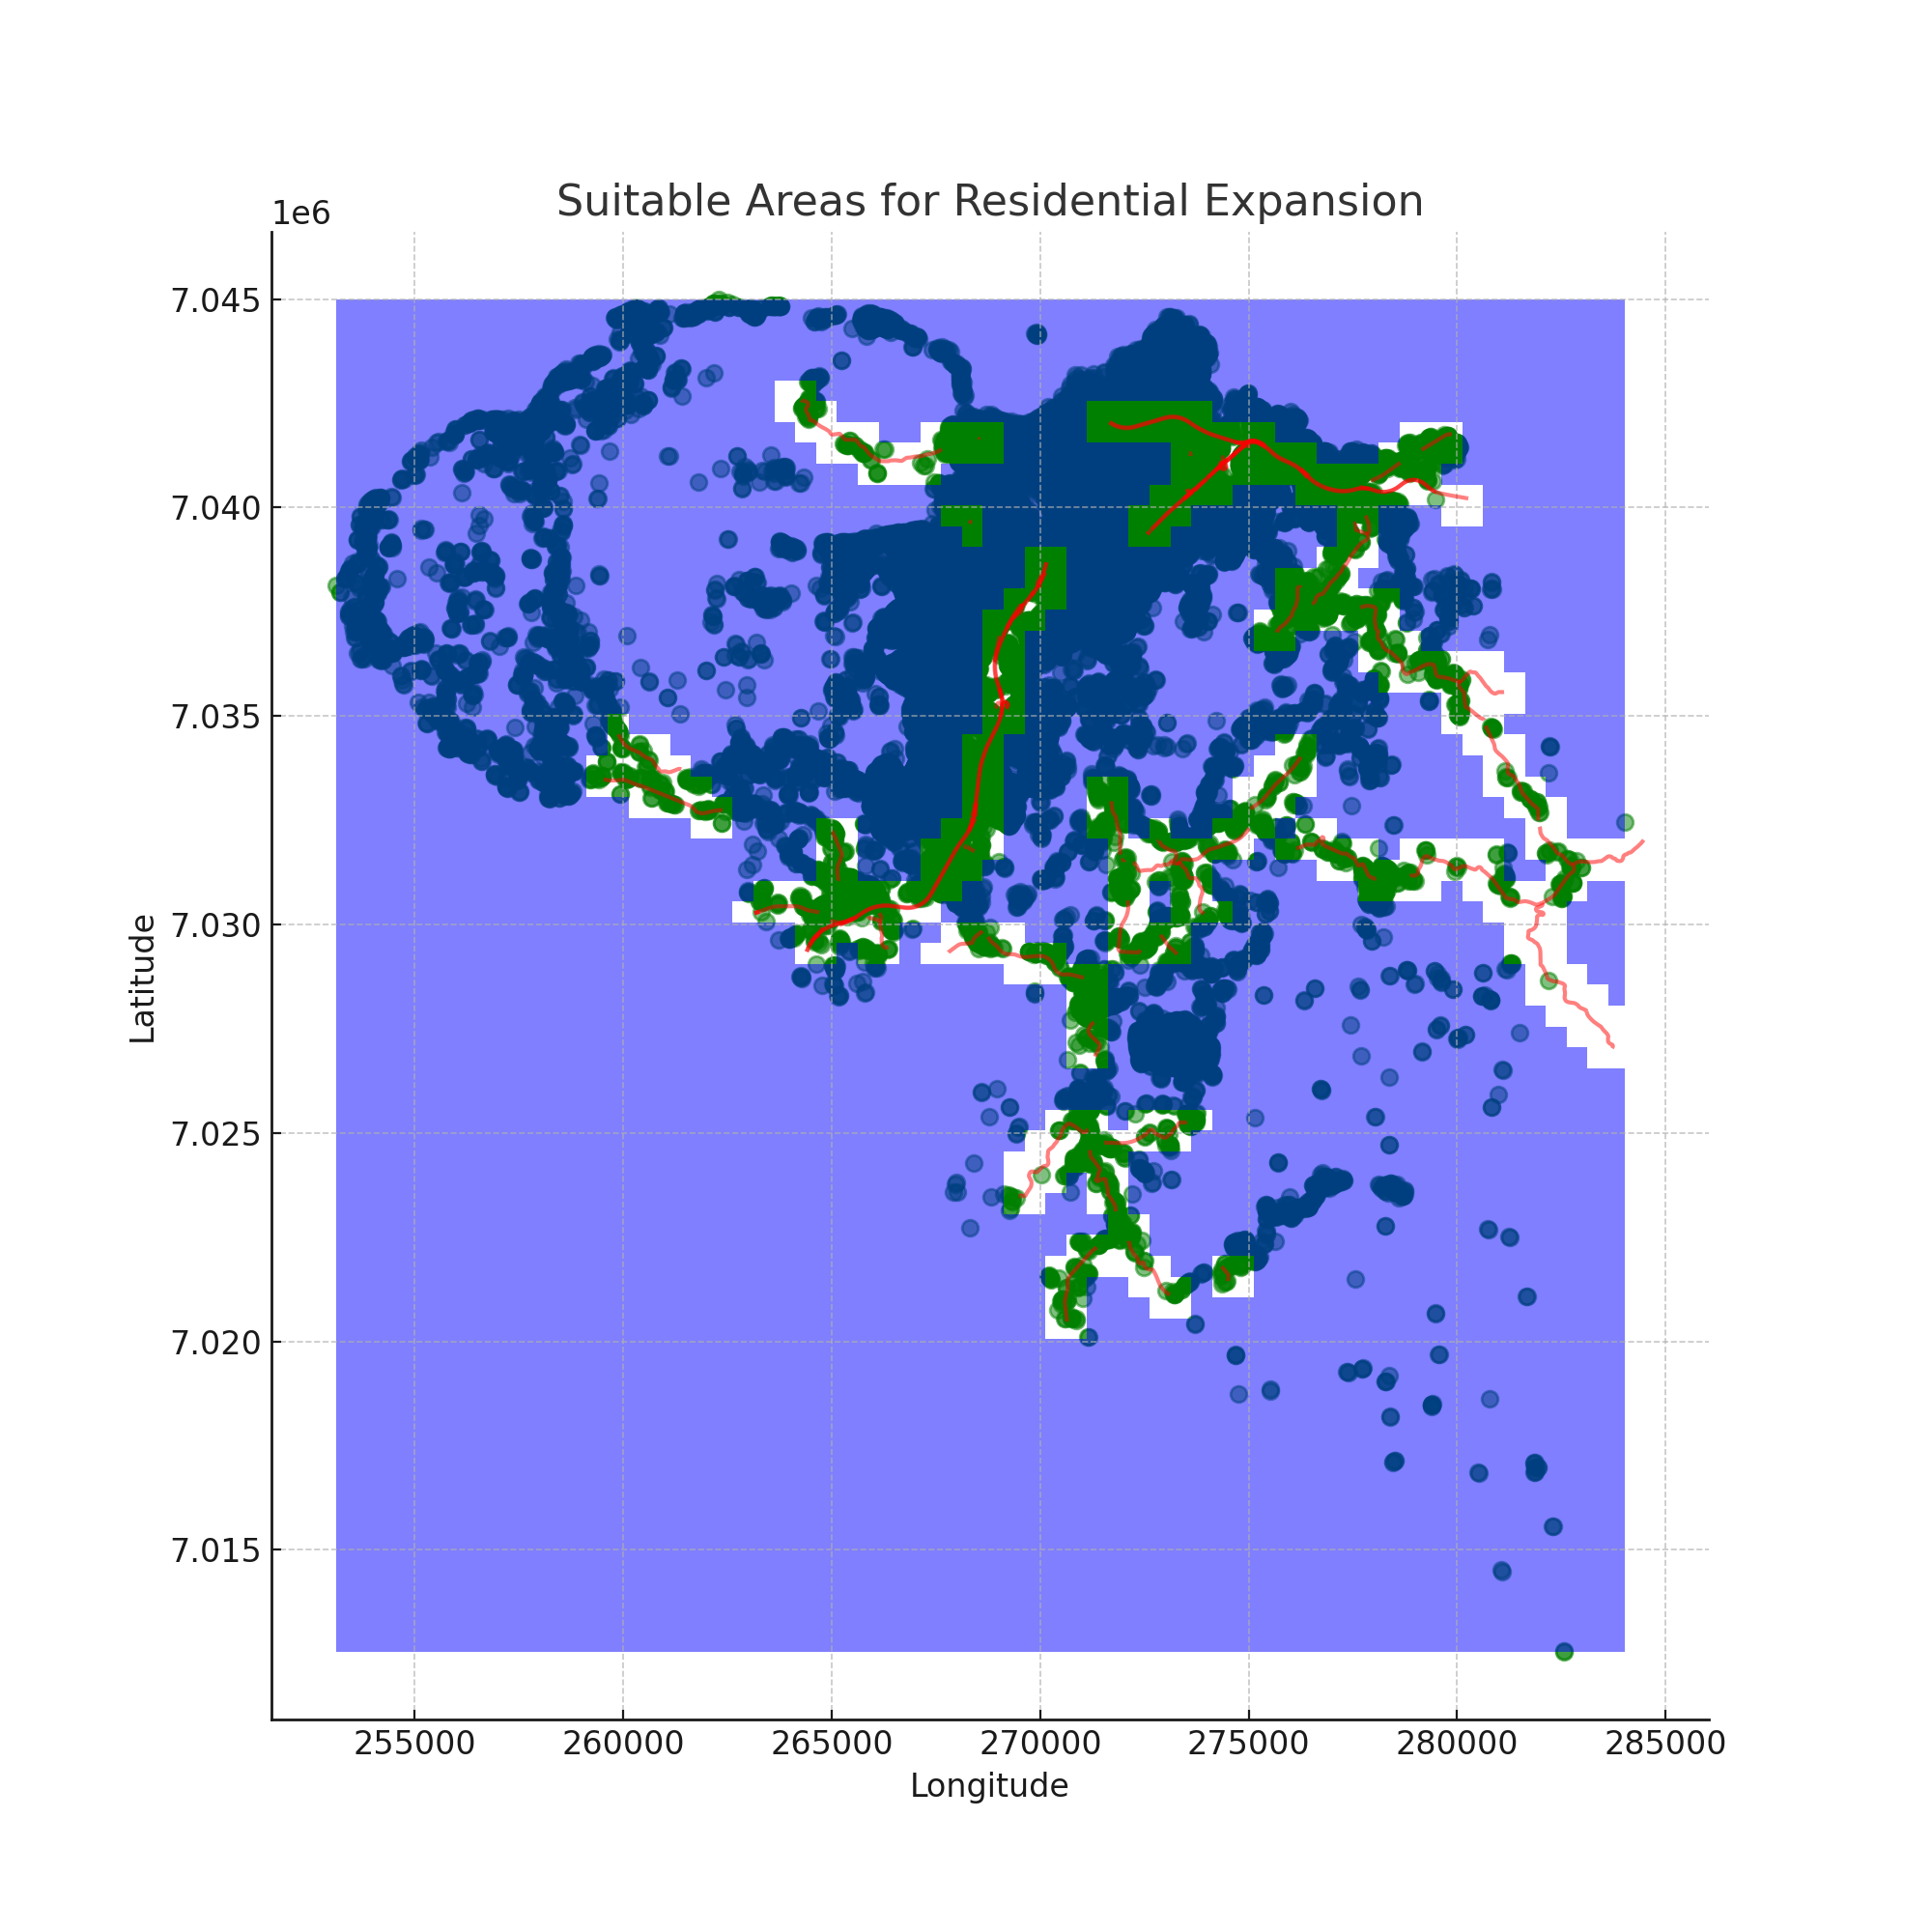
\includegraphics[width=\textwidth]{../figs/residential_expansion_areas_map.png}
    \caption{The result of ChatGPT when asked to \enquote{Find the area best suited for expansion to accommodate residential buildings}, using provided GeoJSON datasets. Potentially suitable areas for residential expansion  are depicted in blue.}
    \label{fig:planning-plot-from-geojson}
\end{figure}

\subsection{Results for Experiment 2}\label{subsec:experiment-2-results}

\autoref{subfig:drammen-outline-file-upload} and \autoref{subfig:drammen-outline-api} shows the results when providing ChatGPT-4 with the GeoJSON for the outline of Drammen municipality using the file upload functionality and providing it and URL to an \acrshort{acr:api} endpoint, respectively. While the Code Interpreter handled the direct file upload with ease, it struggled when provided with the URL to the corresponding web \acrshort{acr:api}. When provided with the URL, its first response was that \enquote{there was a problem with establishing a connection to the website}, after trying to process the request using Code Interpreter. When guided (twice) to try accessing the URL using its web browsing abilities, it was eventually able to read the data. In the subsequent prompt it was asked to provide a visual representation, but failed to do so successfully as \autoref{subfig:drammen-outline-api} shows. The reason for this was its decision to \enquote{truncate the dataset for brevity, using a subset of the full coordinate list} (see \autoref{lst:python-for-failed-drammen-outline}).

\begin{figure}
    \centering
    \begin{subfigure}{0.45\textwidth}
        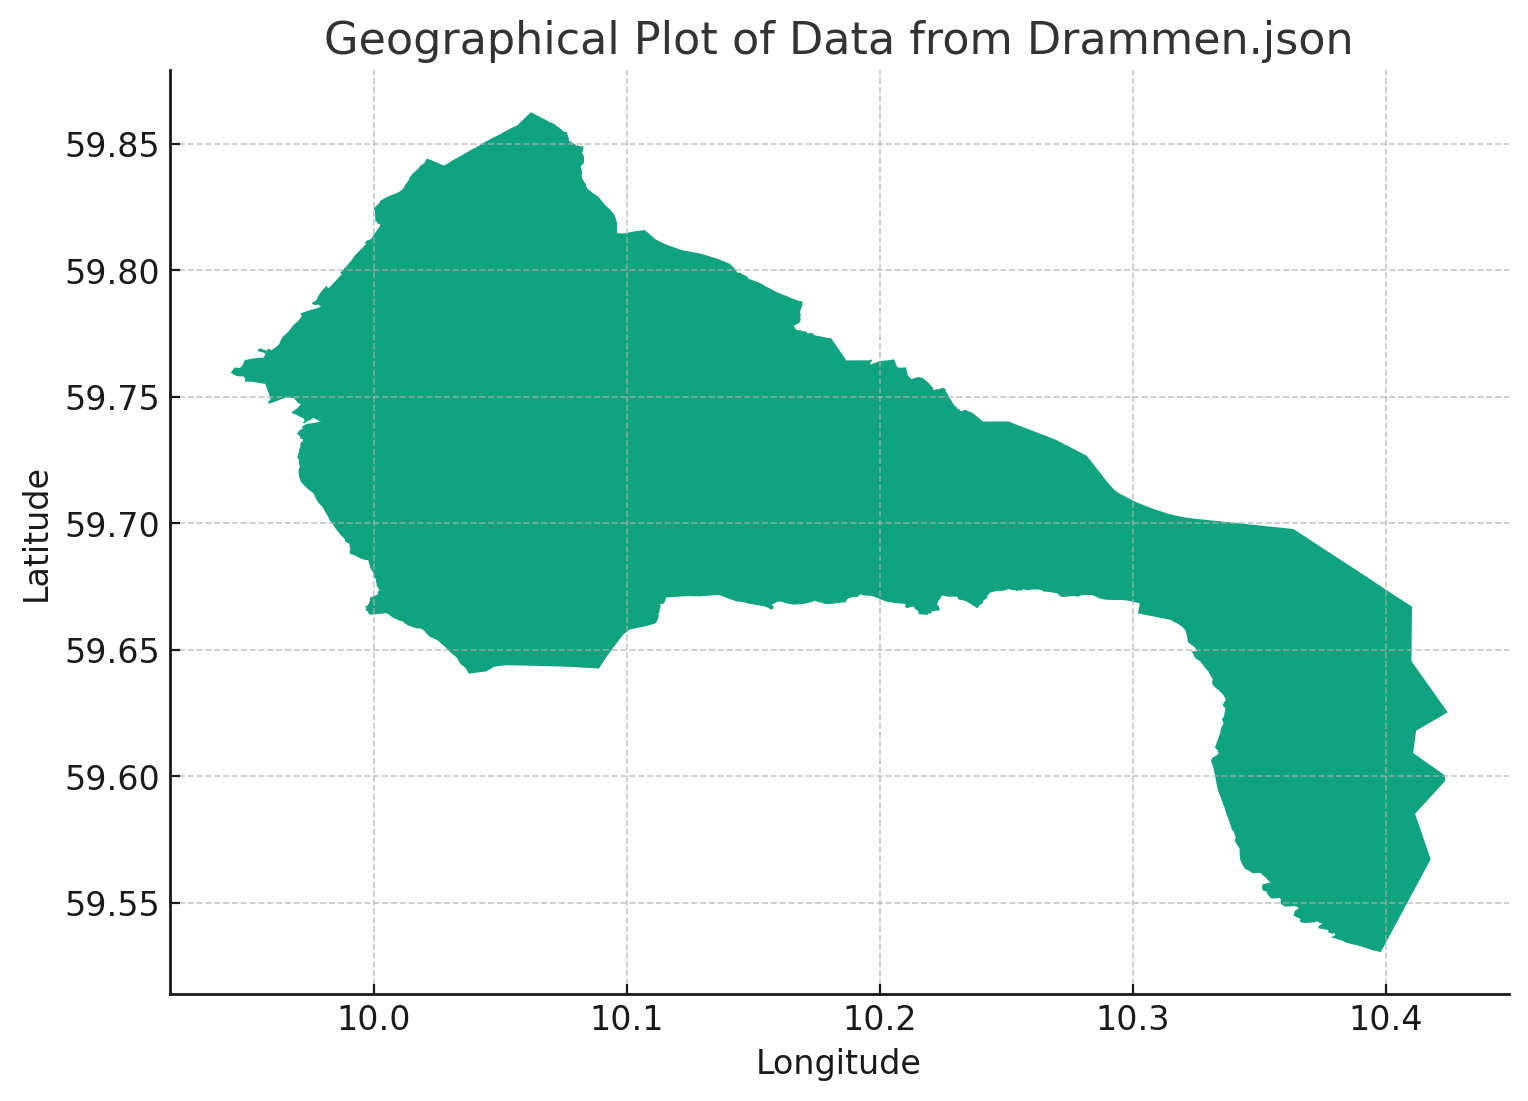
\includegraphics[width=\linewidth]{../figs/drammen_outline_file_upload.png}
        \caption{File upload}
        \label{subfig:drammen-outline-file-upload}
    \end{subfigure}
    \hfill
    \begin{subfigure}{0.45\textwidth}
        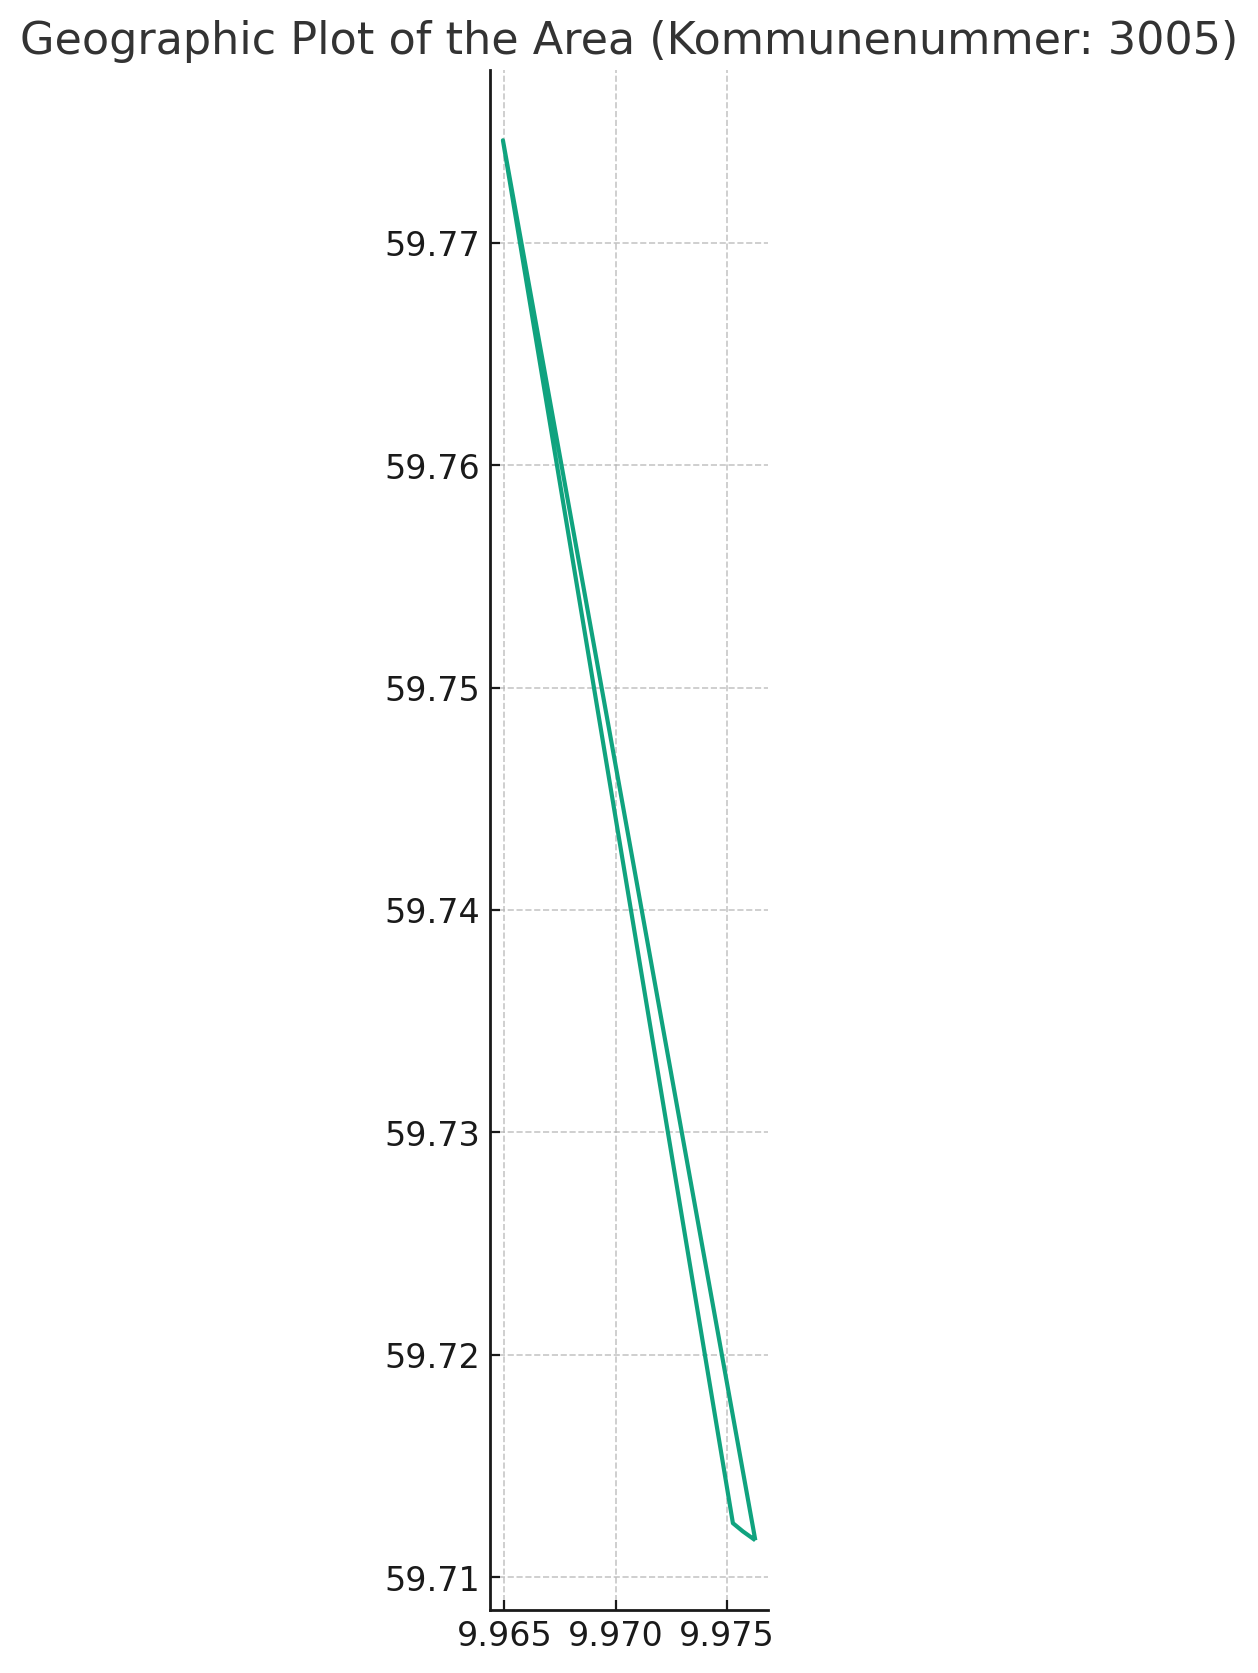
\includegraphics[width=\linewidth]{../figs/drammen_outline_api.png}
        \caption{Providing URL}
        \label{subfig:drammen-outline-api}
    \end{subfigure}
    \caption{Comparison of the resulting outline of Drammen when using file upload (\subref{subfig:drammen-outline-file-upload}) and providing an URL to an API endpoint (\subref{subfig:drammen-outline-api}) with ChatGPT-4}
    \label{fig:file-upload-api-comparison}
\end{figure}

\begin{minipage}{\linewidth}
    \begin{lstlisting}[style=python, caption=ChatGPT code that truncates coordinates, label=lst:python-for-failed-drammen-outline]
# ...

# Extracted coordinates from the JSON data
coordinates = [
    [[9.976278541184014, 59.71166107645171], [9.975715936016496, 59.71206324390201], [9.975270250797282, 59.71243147807226], 
    # ... Truncated for brevity, using a subset of the full coordinate list
    [9.964929990238785, 59.774609947672644]]
]

# ...
\end{lstlisting}
\end{minipage}

\subsection{Results for Experiment 3}\label{subsec:experiment-3-results}

The \texttt{AgentExecutor} with the \texttt{gpt-4-1106-preview} was able to call the two functions in the correct order and with the correct arguments. \autoref{fig:drammen-plot-langchain} show the resulting plot. The notebook used for the experiment is available on the project GitHub repository\footnote{\url{https://github.com/oskarhlm/prosjektoppgave/blob/main/src/python/examples/drammen_ogc_test/drammen_ogc_test.ipynb}}.

\begin{figure}
    \centering
    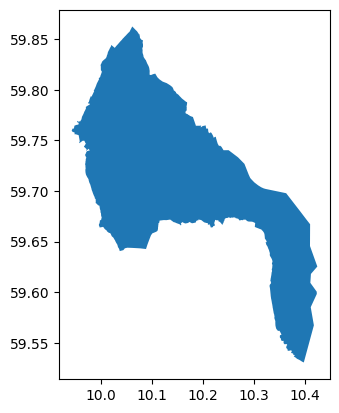
\includegraphics[width=0.4\textwidth]{../figs/drammen_plot_langchain.png}
    \caption{Outline of Drammen using LangChain and OpenAI Functions}
    \label{fig:drammen-plot-langchain}
\end{figure}

\glsresetall

\chapter{Discussion and Conclusion}\label{cha:discussion-and-conclusion}

Sections \ref{sec:code-interpreter-discussion} and \ref{sec:api-access-discussion} will discuss the test results from \autoref{sec:experimental-results} and provide suggestions as to how the limitations highlighted by the tests can be mitigated. \Autosectionref{sec:conclusion-and-future-work} will conclude this specialization project report, and provide directives for future work on the subject of \acrshort{acr:llm}-powered \acrshort{acr:gis}.

\section{Using ChatGPT's Code Interpreter for Geospatial Analysis}\label{sec:code-interpreter-discussion}

When using ChatGPT's built-in Code Interpreter with file uploads, it became apparent that it runs in a Linux environment and utilizes a mounted drive in the \texttt{/mnt} directory, typically used for temporarily mounted filesystems. In an initial test on the \acrshort{acr:sosi} data format, it tried to execute this \acrshort{acr:gdal} command

$$
    \texttt{ogr2ogr -f "GeoJSON" \{converted\_geojson\_path\} \{sosi\_file\_path\}}
$$

\noindent to perform a conversion from \acrshort{acr:sosi} to GeoJSON, the latter of which is far easier to manipulate in a Python environment. This test failed, and the system's response was that \enquote{the \texttt{ogr2ogr} tool is not available in this environment}.

This result was not very surprising, especially since the driver needed to read and write \acrshort{acr:sosi} files---which is called \textit{fyba}\footnote{\url{https://github.com/kartverket/fyba}} and is developed by the Norwegian Mapping Authority---is almost certainly not available in the standard Linux environment used for ChatGPT's Code Interpreter. As the \acrshort{acr:sosi} standard is still widely used for Norwegian geospatial purposes (though according to its Wikipedia page\footnote{\url{https://no.wikipedia.org/wiki/SOSI-formatet}} expected to be exchanged with the \acrshort{acr:gml} format in the future), it is important for an \acrshort{acr:llm}-based \acrshort{acr:gis} agent focused on the Norwegian market to be able to handle this file type.

The inability of flexibly manipulating the Linux environment used by the Code Interpreter then clearly poses some limitations when developing \acrshort{acr:llm}-based systems. A possible solution is to create a custom environment on a server that we control ourselves. Having the \acrshort{acr:ai} agent run in an environment that we have full control over, gives us greater flexibility, and we can then grant the agent access to powerful \acrshort{acr:gis} tooling, such as the \acrshort{acr:gdal} library. The open-source \enquote{Open Interpreter} project \citep{killianlucasKillianLucasOpeninterpreter2023} could prove useful as an alternative to the closed-source Code Interpreter from OpenAI. Open Interpreter lets us run the interpreter on the computer/server of our choosing, so that it can access the file system directly, as well as libraries and programs stored on the computer/server. It also allows for other \acrshortpl{acr:llm} than \acrshort{acr:gpt}-4, such as Mistral \acrshortpl{acr:llm} and Code-LLaMA. Additionally, with it being an open-source project, one can \enquote{fork} the repository and make project-specific modifications to the interpreter.

\section[Mitigating ChatGPT's Inability to Access Web APIs]{Mitigating ChatGPT's Inability to Access Web \acrshort{acr:api}s}\label{sec:api-access-discussion}

As the results from Test 2 (see \autoref{subsec:experiment-2-results}) show, ChatGPT-4 struggles when provided with URLs to external web \acrshortpl{acr:api}, even when prompted to use its web browsing capabilities and pairing them with its Code Interpreter. These issues are not present when using direct file upload, in which case the model appears to save the uploaded file in a temporary file directory in its Linux environment. Interpreting the inner workings of the Code Interpreter from the code samples in the chat can be challenging, but it appears that it does not do this by default after fetching data from an external web \acrshort{acr:api}. As \autoref{lst:python-for-failed-drammen-outline} shows, it \textit{truncates} the file contents and \enquote{stores} them directly in the code, in an attempt to keep the entire file contents within the context window of the \acrshort{acr:llm}. The context window of the ChatGPT-4 model is currently at 32,000 tokens, and the new GPT-4 Turbo has a context length of 128,000 tokens. While these are of significant size, they are not meant to (or able to) store large file. The size of the context window therefore becomes a limiting factor when the file contents grow large, which is not uncommon for geospatial files.

This is a significant limitation of using ChatGPT-4 out of the box, and one should therefore look into other ways of handling web requests and subsequent storing of the received data. Techniques within \gls{acr:rag}, and libraries like LangChain and Open Interpreter, could help solve this issue.

\glsresetall

\section{Conclusion and Future Work}\label{sec:conclusion-and-future-work}

This specialization project report has presented a literature study in the fields of \acrlong{acr:nlp}, \acrlongpl{acr:llm}, \acrshort{acr:gis}, planning for \acrshortpl{acr:llm}, and \acrlong{acr:rag}, along with three tests that try to demonstrate strengths and weaknesses of \acrshortpl{acr:llm} when dealing with geospatial data. The literature study and tests serve to provide a better starting point when attempting to develop \acrshort{acr:llm}-based \acrshort{acr:gis} agents.

One important finding of the literature study is that there has been a substantial body of work done concerning the potential of using \acrlongpl{acr:llm} in \acrshort{acr:gis} analysis (see \autoref{sec:gis-with-llms}). Studies have been conducted to show that the \acrshort{acr:gpt}-4 model has good geospatial awareness, and there have been created a number of prototypes of autonomous \acrshort{acr:gis} systems powered by \acrshortpl{acr:llm}. \Autosectionref{sec:planning-strategies} discussed various planning strategies that have been developed to facilitate better decision making and reasoning in \acrshort{acr:llm}-based systems. \Autosectionref{sec:retrieval-automented-generation} introduced \gls{acr:rag}, the concept of providing \acrshortpl{acr:llm} with access to external tooling to help them produce informed and up-to-date responses.

The three tests showcased \acrshort{acr:gpt}-4's abilities of handling geospatial data using various data formats and access channels. The results from Test 1 and 2 showed that it has \textit{some} understanding of how to perform geospatial analysis, but that it also has substantial limitations, e.g., reading and writing large files and accessing data through web \acrshortpl{acr:api}. Test 3 (see \autoref{subsec:ex-3-setup}) served as an initial test of utilizing tools such as LangChain to extend the capabilities of \acrshortpl{acr:llm} like \acrshort{acr:gpt}-4 through programmatic methods.

With this being a specialization project that will transition into a larger master thesis, some points of discussion have been reserved for future work. Additionally, the task of developing a proof of concept has been assigned to the master thesis due to time constraints and the intention to acquire more knowledge before proceeding with development. Subsections \ref{subsec:memory-and-embeddings} and \ref{subsec:testing-regime} will elaborate upon potentially important issues that should be addressed when developing \acrshort{acr:llm}-based \acrshort{acr:gis} agents.

% \subsection{Balancing Accuracy Against Performance and Costs}

% The ecosystem of agent frameworks and planning strategies to improve agent performance on complex tasks (discussed in \nameref{cha:related-work}), is a growing one. Different agents frameworks and planning strategies should be compared to see which are most viable for \acrshort{acr:gis} work. Important considerations are the ability to destructure complex problems, the ability to take advantage of external tooling, and computational time. More complex planning strategies typically demand more interactions with \acrshort{acr:llm} \acrshortpl{acr:api}, which can be expensive both in terms of computational time and cost (when using a monetized \acrshort{acr:api} like OpenAI's for \acrshort{acr:gpt}-4 and \acrshort{acr:gpt}-4).

% \cite{clearyLatencyBenchmarksComparisons2023} did benchmarking of different \acrshortpl{acr:llm} on different providers. Important takeaways were that \acrshort{acr:gpt}-4 is about 6.3 times slower than \acrshort{acr:gpt}-3.5-Instruct, and that Azure has far lower latency in most cases for inference on \acrshort{acr:gpt} models. Such considerations are important when addressing usability of \acrshort{acr:llm}-based applications, balancing accuracy against speed and cost. Using free open-source alternatives where possible is a good option to reduce cost. Open-source software like the Open Interpreter project should also be investigated.

\subsection{Memory and Embeddings}\label{subsec:memory-and-embeddings}

Storing information for future use is important when developing \acrshort{acr:llm}-based agents in order for them to produce consistent responses. \cite{wengLLMPoweredAutonomous2023} presents three different types of memory in human brains: (1) \textit{Sensory Memory}, (2) \textit{Short-Term Memory}, and (3) \textit{Long-Term Memory}. When translated to \acrshortpl{acr:llm}, we can think of \textit{Sensory Memory} as learning embedding representations, \textit{Short-Term Memory} as the memory contained within the limits of the context window of the Transformer, and  \textit{Long-Term Memory} as an external vector store that can be attended to by the agent at query time. Such a vector store/database would store the vector embeddings of the data contained within it, and allow for fast and accurate similarity search and retrieval based on the vector distance or similarity between the vector representations \citep{evchakiVectorDatabase2023}. \cite{wengLLMPoweredAutonomous2023} lists some common approximate nearest neighbours algorithms for fast retrieval speeds, including \gls{acr:lsh} and \gls{acr:faiss}.

Future work should build upon the research of \cite{unluChatmapLargeLanguage2023} (see \autoref{sec:gis-with-llms}) and investigate whether vector embeddings can be utilized for long-term storage of geospatial data with textual descriptions, or if a vector database can efficiently retrieve relevant resources such as \acrshortpl{acr:api} or other external tools based on their documentation/specifications. Furthermore, these documentations and \acrshort{acr:api} specifications can be large is size, and the context length could become a limiting issue. Vector embeddings can help mitigate such issues. By splitting the documents into chunks and indexing them using vector embeddings, one can extract only the relevant parts and pass these to the \acrshort{acr:llm} with the prompt.

\subsection{Testing Regime}\label{subsec:testing-regime}

In order to test the feasibility of different language models to serve as the brain of an autonomous \acrshort{acr:gis} agent, a testing regime should be developed. In the examples of autonomous \acrshort{acr:gis} agents described in the literature study of this report (see \autoref{sec:gis-with-llms}), results were generally presented in the form of case studies. This type of qualitative testing is entirely appropriate for showcasing the possibilities of the technologies, but it may be insufficient for comparing the performance of \textit{different} systems. A quantitative approach would probably be preferable.

One idea is to create a test dataset which consists of inputs and corresponding desired outputs of typical \acrshort{acr:gis} tasks. Inputs would in this case be natural language queries inputted by a mock user, and the outputs would be what you would expect a \acrshort{acr:gis} professional to return when given the same tasks/queries. Inputs should reflect the varying level of \acrshort{acr:gis} knowledge between different user groups (see \autoref{sec:user-groups}). Outputs could be files with typical geospatial extensions (.shp, .geojson, .sos, etc.), or they could adhere to API specifications from geospatial standards (see \autoref{sec:geospatial-standards}).

While the inputs should be fairly simple to construct, there are several questions to be answered in regard to the outputs, among which are the following:

\begin{itemize}
    \item How does one evaluate the accuracy of the output?
    \item How should the \acrshort{acr:ai} agent respond when the user does not specify an output file format?
    \item How does one evaluate the usefulness of responses to questions that should \textit{not} return geospatial files, e.g., answers to general questions about geo-related subjects?
\end{itemize}

\noindent These questions are outside the scope of this specialization project, and are therefore left out for future work.



\glsaddall

%%%%%%%%%%%%%%%%%%%%%%%%%%%%%%%%%%%%%%%%%%%%%%%%%%%%%
%\backmatter
\clearpage
\phantomsection
\addcontentsline{toc}{chapter}{Bibliography}
\printbibliography

\appendix

\chapter*{Appendices}
\label{cha:appendices}
\addcontentsline{toc}{chapter}{Appendices}

\begin{comment}
\chapter{Proof of the First Zonklar Equation}
\label{app:zonklar}

Appendix one text goes here.

\chapter{Structured Literature Review (SLR) Protocol}
\label{app:slr}

Appendix two text goes here.
\end{comment}

\includeappendixpdfwithtitle{Task Description from Norkart}{appendices/project_description.pdf}
% \includeappendixpdf{2}{appendices/project_description.pdf}


\clearpage
\printglossary[type=\acronymtype]

\end{document}
